@@ -62,6 +62,8 @@
\newcommand{\R}{\mathbb{R}}
\newcommand{\ZZ}{\mathbb{Z}}
\newcommand{\N}{\mathbb{N}}
\newcommand{\zz}{\mathbb{Z}}
\newcommand{\nn}{\mathbb{N}}
\newcommand{\m}[1]{\mathcal{#1}}
\newcommand{\id}{\textrm{id}}
\newcommand{\un}{\underline}
@ -100,6 +102,7 @@
\newcommand{\cat}{\ensuremath{\mb{Cat}}}
\newcommand{\epz}{\varepsilon}
\newcommand{\Alg}{\mbox{-}\mb{Alg}}
\newcommand{\morln}{\morln}
\newcolumntype{L}{>{$}l<{$}}
\newcolumntype{C}{>{$}c<{$}}
\newcolumntype{R}{>{$}r<{$}}
@ -186,8 +189,8 @@

The goal of this chapter will be to show that we can reconstruct all of the morphisms of $L_n$ from the abelian group $\mathrm{M}(L_n)^{\mathrm{gp, ab}}$, and therefore that we can actually use the adjunction from \cref{Moradj} to help find a description of the free $E\Lambda$-algebra on $n$ invertible objects. 

The first step towards this goal will involve splitting $\mathrm{Mor}(L_n)$ up as the product of two other monoids. The first of these will encode all of the possible combinations of source and target data for morphisms in $L_n$, while the second will just be the endomorphisms of the unit object, $L_n(I, I)$. 
Once we have done this, we can then use the fact that $L_n(I, I)$ is always an abelian group to rewrite $\mathrm{Mor}(L_n)$ in terms of its abelian group completion, $\mathrm{Mor}(L_n)^{\mathrm{gp, ab}}$. This is not quite the same thing as $\mathrm{M}(L_n)^{\mathrm{gp, ab}}$, but they are close enough that we can find a simple equation linking the two, which will in turn allow us to frame the former in terms of the quotient of $\mathrm{M}(\ELnn)^{\mathrm{gp, ab}}$ we described last chapter. All together, this will constitute an expression for $\mathrm{Mor}(L_n)$ that is built up of pieces which we know how to calculate.
The first step towards this goal will involve splitting $\morln$ up as the product of two other monoids. The first of these will encode all of the possible combinations of source and target data for morphisms in $L_n$, while the second will just be the endomorphisms of the unit object, $L_n(I, I)$. 
Once we have done this, we can then use the fact that $L_n(I, I)$ is always an abelian group to rewrite $\morln$ in terms of its abelian group completion, $\morln^{\mathrm{gp, ab}}$. This is not quite the same thing as $\mathrm{M}(L_n)^{\mathrm{gp, ab}}$, but they are close enough that we can find a simple equation linking the two, which will in turn allow us to frame the former in terms of the quotient of $\mathrm{M}(\ELnn)^{\mathrm{gp, ab}}$ we described last chapter. All together, this will constitute an expression for $\morln$ that is built up of pieces which we know how to calculate.

Current understanding is four steps:
\begin{enumerate}
@ -403,7 +406,7 @@ By the interchange law for monoidal categories,
\]
\end{proof} 

Thus in cases where every object of $X$ is invertible, the monoidal structure together with knowledge of each morphism's source and target will be enough to determine $X$ uniquely. Since all objects in $L_n$ are invertible, this means that we could choose to ignore composition of elements of $\mathrm{Mor}(L_n)$ QQQ this should have had a notation environment a long time ago QQQ for the time being, and focus on its status as a monoid under tensor product.
Thus in cases where every object of $X$ is invertible, the monoidal structure together with knowledge of each morphism's source and target will be enough to determine $X$ uniquely. Since all objects in $L_n$ are invertible, this means that we could choose to ignore composition of elements of $\morln$ for the time being, and focus on its status as a monoid under tensor product.



@ -453,7 +456,7 @@ For a commutative monoid $A$, it is clear that $M(BA)^{ab} = A$, so we can defin

\begin{enumerate}
\item Our goal was to have an adjunction involving $\lmc$, not $\moncat$, since we want to apply it to strict $\ML$-monoidal functors instead of arbitrary strict monoidal functors. 
\item Even if we do find a way to use this adjunction to extract information about $L_n$, it will not be the monoid $\mathrm{Mor}(L_n)$ we were originally after, only a strange abelianized version where tensor product and composition coincide.  
\item Even if we do find a way to use this adjunction to extract information about $L_n$, it will not be the monoid $\morln$ we were originally after, only a strange abelianized version where tensor product and composition coincide.  
\end{enumerate} 

Unfortunately, this adjunction seems to be the best that we can do. 
@ -645,10 +648,44 @@ Let $f$ be an arbitrary morphism in $L_n$. By surjectivity of $q$, there must ex

Note that while this result shows that every morphism of $L_n$ is induced by the action of some $g \in \Lambda(m)$, it does not imply that this $g$ is unique.

<<<<<<< Updated upstream
\begin{conv}
The monoid homomorphism $\mathrm{Ob}(q)  :  \mathbb{N}^{\ast 2n}  \to  \mathbb{Z}^{\ast n}$ has a canonical section $q^{-1}$ given as follows. An element $w \in \mathbb{Z}^{* n}$ can be written as a word in $z_i, z_i^*$ in normal form, that is in the fewest number of symbols. We define $q^{-1}(z_i) = z_i$ and $q^{-1}(z_i^*) = z_{n+i}$, and then 
\[
q^{-1}(w) = q^{-1}(w_1) \cdots q^{-1}(w_k)
=======
Note that while this result shows that every morphism of $L_n$ is induced by the action of some $g \in \Lambda(m)$, it does not imply that this $g$ is unique. It will, however, furnish us with all the group actions required to give $L_n$ a $\ML$-monoidal structure once we have given it a mere \emph{monoidal} one using that $q$ is surjective (\cref{qsurj}).  

\begin{lem} \label{noscalar} For any element $g \in \Lambda(m), m \in \mathbb{N}$ of an action operad $\ML$, the morphism
\[
g: I^m \to I^m
\]
in $L_n$ is the identity.
Equivalently, for any element $h \in \Lambda(0)$, $h$ induces the identity morphism $I \to I$.
\end{lem}

\begin{proof}
First, let $g \in \Lambda(m)$. Then $g: I^m \to I^m$ is equal to $q(g):q(I^m) \to q(I^m)$ which is equal to $q\delta(g): q\delta(I^m) \to q\delta(I^m)$. Since $q$ is the coequalizer of $\delta$ and the zero map, $q\delta(g) = \id$ for all $g \in \Lambda(m)$. This clearly implies that every $h \in \Lambda(0)$ induces the identity map $I \to I$, but note that the morphism $g:I^m \to I^m$ is also the morphism induced by $\mu(g; e_0, \ldots, e_0) \in \Lambda(0)$, so these two claims are equivalent.
\end{proof}

This is a curious result. The morphisms $I \to I$ in QQQ $n\ML$ vs $\ELn$ QQQ are exactly the elements of the group $\Lambda(0)$, but all of these become the identity in $L_n$. In other words, $L_n$ cannot detect any morphisms in $\Lambda(0)$, an idea we make precise now. 


\begin{prop} \label{G0quot} Let $\Lambda$ be a crossed action operad. Then there exists another crossed action operad $\Lambda'$ given by $\Lambda'(m) = \Lambda(m)/\Lambda(0)$ for all $m \in \mathrm{N}$.
\end{prop}
\begin{proof}
For any elements $g \in \Lambda(m)$ and $h \in \Lambda(0)$, their tensor product $h \otimes g := \mu(e_2; h, g)$ is also an element of $\Lambda(m)$. This defines a map $\Lambda(0) \times \Lambda(m) \to \Lambda(m)$, which is both a group homomorphism and a group action by \cref{G0abel}. This produces a homomorphism $\Lambda(0) \to \Lambda(m)$ for all $m$ which lies in the center of $\Lambda(m)$ by QQQ \cref{spacial}, hence is normal for all $m$. Furthermore, the induced map $\Lambda(0) \to \Lambda(m) \to \Sigma_m$ is the zero map, so we have an induced homomorphism $\Lambda(m)/\Lambda(0) \to \Sigma_m$. All that remains to be shown is that we the operadic multiplication for $\Lambda$ induces one for the groups $\Lambda(n)/\Lambda(0)$, and that this multiplication satisfies the axioms for an action operad.

Let $h, h_1, ..., h_m \in \Lambda(0)$ and $k_1, ..., k_m \in \mathbb{N}$. We have the following calculation using the action operad axioms for $\Lambda$ and the fact that $\EL(\underline{1})$ is spacial (see \cref{spacial}) so the $e_k$ commute with all elements of $\Lambda(0)$.
\[ \begin{array}{rll}
		\mu^{\Lambda}( \, h \otimes e_m \, ; \, h_1 \otimes e_{k_1}, ..., h_m \otimes e_{k_m} \, ) & = & \mu^{\Lambda}\big( \, \mu^{\Lambda}(e_2; h, e_m) \, ; \, h_1 \otimes e_{k_1}, ..., h_m \otimes e_{k_m} \, \big) \\
		& = & \mu^{\Lambda}\big( \, e_2 \, ; \, \mu^{\Lambda}(h;-), \mu^{\Lambda}(e_m; h_1 \otimes e_{k_1}, ..., h_m \otimes e_{k_m}) \, \big) \\
		& = & \mu^{\Lambda}(h;-) \otimes \mu^{\Lambda}(e_m; h_1 \otimes e_{k_1}, ..., h_m \otimes e_{k_m})  \\
		& = & h \otimes h_1 \otimes e_{k_1} \otimes ... \otimes h_m \otimes e_{k_m} \\
		& = & e_{k_1} \otimes ... \otimes e_{k_m} \otimes h \otimes h_1 ... \otimes h_m \\
		& = & e_{k_1+...+k_m} \otimes h \otimes h_1 ... \otimes h_m
		\end{array}
>>>>>>> Stashed changes
\]
where $w = w_1 \cdots w_k$ is the normal form of $w$. We note that $q^{-1}$ is merely a function, and not a monoid homomorphism.
\end{conv}
@ -813,7 +850,7 @@ Recalling \cref{Gnobj,Gnconcomp,Zobj,crossconcomp}, we can immediately conclude
where the pullbacks are taken over the quotients of abelianization for $(\mathbb{N}^{\ast n})^{\mathrm{ab}} = \mathbb{N}^n$ and $(\mathbb{Z}^{\ast n})^{\mathrm{ab}} = \mathbb{Z}^n$ respectively.
\end{cor}

Next, we want to show that this $(s \times t)(L_n)$ we have described is in fact a submonoid of $\mathrm{Mor}(L_n)$.  We will accomplish this  by first proving the analogous statement for all $\ELn$, and then recovering the $L_n$ version from it later.  For any pair $(w, w') \in \mathbb{N}^{\ast n} \times_{\mathbb{N}^n} \mathbb{N}^{\ast n}$ such that the images of $w$ and $w'$ in the commutative monoid $\mathbb{N}^n$ are the same, there are generators $x_1, ..., x_m$ for which 
Next, we want to show that this $(s \times t)(L_n)$ we have described is in fact a submonoid of $\morln$.  We will accomplish this  by first proving the analogous statement for all $\ELn$, and then recovering the $L_n$ version from it later.  For any pair $(w, w') \in \mathbb{N}^{\ast n} \times_{\mathbb{N}^n} \mathbb{N}^{\ast n}$ such that the images of $w$ and $w'$ in the commutative monoid $\mathbb{N}^n$ are the same, there are generators $x_1, ..., x_m$ for which 
\[ w \quad = \quad x_1 \otimes ... \otimes x_m \]
and there exists at least one permutation $\sigma \in S_m$ such that
\[ w' \quad = \quad x_{\sigma(1)} \otimes ... \otimes x_{\sigma(m)}. \]
@ -836,16 +873,16 @@ and being an element of the pullback immediately implies $k=j$. We then define a
\[
(w,w') = c_1 \cdots c_s = d_1 \cdots d_t,
\]
then the length (QQQ we defined this kind of thing somewhere) of $c_1$ must be either strictly less than or strictly greater than the length of $d_1$; if they had equal length, then they would be equal. Without loss of generality assume $c_1$ has length $l_c$ which is strictly less than the length $l_d$ of $d_1$. But then the first $l_c$ terms appearing in $d_1$ would agree with $c_1$, proving that $d_1$ is not indecomposable. Straightforward induction then finishes the proof that every element of $\mathbb{N}^{\ast n} \times_{\mathbb{N}^n} \mathbb{N}^{\ast n}$ can be written as a product of indecomposables in a unique way, making $\mathbb{N}^{\ast n} \times_{\mathbb{N}^n} \mathbb{N}^{\ast n}$ free on the set of indecomposables.
then the length of $c_1$, as defined in Proposition \ref{Gfree}, must be either strictly less than or strictly greater than the length of $d_1$; if they had equal length, then they would be equal. Without loss of generality assume $c_1$ has length $l_c$ which is strictly less than the length $l_d$ of $d_1$. But then the first $l_c$ terms appearing in $d_1$ would agree with $c_1$, proving that $d_1$ is not indecomposable. Straightforward induction then finishes the proof that every element of $\mathbb{N}^{\ast n} \times_{\mathbb{N}^n} \mathbb{N}^{\ast n}$ can be written as a product of indecomposables in a unique way, making $\mathbb{N}^{\ast n} \times_{\mathbb{N}^n} \mathbb{N}^{\ast n}$ free on the set of indecomposables.
\end{proof}

We can now construct the desired injection using the function $\rho$ from \cref{rho_ww'}.
\begin{prop} \label{stGnsub} $\mathrm{Mor}(\ELn) \to (s \times t)(\ELn)$ is a split epi of monoids, so $(s \times t)(\ELn)$ is (isomorphic to) a submonoid of $\mathrm{Mor}(\ELn)$. Furthermore, we can choose the injection $i:(s \times t)(\ELn) \to \mathrm{Mor}(\ELn)$ such that the following diagram commutes.
\begin{center}
    \begin{tikzpicture}[x=20mm,y=15mm]
    \begin{tikzpicture}[x=30mm,y=15mm]
		\node (a) at (0,0) {$\mathrm{Ob}(\ELn)$};
		\node (b) at (1,0) {$(s \times t)(\ELn)$};
		\node (d) at (1,-1) {$\mathrm{Mor}(\ELn)$};
		\node (b) at (10,0) {$(s \times t)(\ELn)$};
		\node (d) at (10,-10) {$\mathrm{Mor}(\ELn)$};
      \draw [->] (a) to (b);
			\draw [->] (a) to node [above] {$$} (b);
			\draw [->] (b) to node [right] {$i$} (d);
@ -900,12 +937,12 @@ The first statement follows immediately from the injectivity of $\delta$ on obje
\end{proof}


\begin{prop} \label{stZsub} $\mathrm{Mor}(L_n) \to (s \times t)(L_n)$ is a split epi of monoids, so $(s \times t)(L_n)$ is (isomorphic to) a submonoid of $\mathrm{Mor}(L_n)$. Furthermore, we can choose the injection $i:(s \times t)(L_n) \to \mathrm{Mor}(L_n)$ such that the following diagram commutes.
\begin{prop} \label{stZsub} $\morln \to (s \times t)(L_n)$ is a split epi of monoids, so $(s \times t)(L_n)$ is (isomorphic to) a submonoid of $\morln$. Furthermore, we can choose the injection $i:(s \times t)(L_n) \to \morln$ such that the following diagram commutes.
\begin{center}
    \begin{tikzpicture}[x=20mm,y=15mm]
		\node (a) at (0,0) {$\mathrm{Ob}(L_n)$};
		\node (b) at (1,0) {$(s \times t)(L_n)$};
		\node (d) at (1,-1) {$\mathrm{Mor}(L_n)$};
		\node (d) at (1,-1) {$\morln$};
      \draw [->] (a) to (b);
			\draw [->] (a) to node [above] {$$} (b);
			\draw [->] (b) to node [right] {$i$} (d);
@ -935,26 +972,26 @@ Furthermore, $(v,v')$ cannot be written as $\delta(u,u')$ for any indecomposable

The functor $q:\ELnn \to L_n$ is the cokernel of $\delta$, so the composite
\[
\mathrm{Mor}(\ELnn) \stackrel{\mathrm{Mor}\delta}{\longrightarrow} \mathrm{Mor}(\ELnn) \stackrel{\mathrm{Mor}q}{\longrightarrow} \mathrm{Mor}(L_n)
\mathrm{Mor}(\ELnn) \stackrel{\mathrm{Mor}\delta}{\longrightarrow} \mathrm{Mor}(\ELnn) \stackrel{\mathrm{Mor}q}{\longrightarrow} \morln
\]
is the zero map. From the definition of $\delta$ in \cref{qdef} and the description of the monoids $(s \times t)(\ELn), (s \times t)(L_n)$ in \cref{stpullback}, the composite
\[
(s \times t)(\ELnn) \stackrel{(s \times t)(\delta)}{\longrightarrow}  (s \times t)(\ELnn) \stackrel{(s \times t)(q)}{\longrightarrow} (s \times t)(L_n)
\]
exhibits $(s \times t)(L_n)$ as the cokernel of $(s \times t)(\delta)$ which induces a unique monoid homomorphism $i: (s \times t)(L_n) \to \mathrm{Mor}(L_n)$ making the square below commute.
exhibits $(s \times t)(L_n)$ as the cokernel of $(s \times t)(\delta)$ which induces a unique monoid homomorphism $i: (s \times t)(L_n) \to \morln$ making the square below commute.
\begin{center}
    \begin{tikzpicture}[x=20mm,y=15mm]
		\node (a) at (0,0) {$(s \times t)(\ELnn)$};
		\node (b) at (2,0) {$\mathrm{Mor}(\ELnn)$};
		\node (c) at (0,-1) {$(s \times t)(L_n) $};
		\node (d) at (2,-1) {$\mathrm{Mor}(L_n)$};
		\node (d) at (2,-1) {$\morln$};
			\draw [->] (a) to node [above] {$i$} (b);
			\draw [->] (b) to node [right] {$q$} (d);
			\draw [->] (a) to node [left] {$q$} (c);
			\draw [->] (c) to node [below] {$i$} (d);
    \end{tikzpicture}
\end{center}
This homomorphism $i$ splits $\mathrm{Mor}(L_n) \to (s \times t)(L_n)$ as desired.
This homomorphism $i$ splits $\morln \to (s \times t)(L_n)$ as desired.

The final claim about commuting with the inclusion of objects follows using the same argument as in  \cref{stGnsub}, so we must also require $\rho(x_i, x_i) = e_1$.

@ -962,13 +999,14 @@ The final claim about commuting with the inclusion of objects follows using the

\section{Unit endomorphisms of \texorpdfstring{$L_n$}{L_n}}

We now consider the monoid of unit endomorphisms, $L_n(I,I)$. This is a particularly important submonoid of the morphisms $\mathrm{Mor}(L_n)$, since it is the only submonoid which is also a homset of the category $L_n$. Moreover, because the maps in $L_n(I,I)$ all share the same source and target, what we have is not just a monoid under tensor product but also under composition as well. This fact leads to a series of special properties for $L_n(I,I)$, the first of which is just another instance of the classic Eckmann-Hilton argument. QQQ Reference here?
We now consider the monoid of unit endomorphisms, $L_n(I,I)$. This is a particularly important submonoid of the morphisms $\morln$, since it is the only submonoid which is also a homset of the category $L_n$. Moreover, because the maps in $L_n(I,I)$ all share the same source and target, what we have is not just a monoid under tensor product but also under composition as well. This fact leads to a series of special properties for $L_n(I,I)$, the first of which is just another instance of the classic Eckmann-Hilton argument. QQQ Reference here?

\begin{prop} \label{endcom} $L_n(I,I)$ is a commutative monoid under both tensor product and composition, with $f \otimes f' = f \circ f'$. Since $L_n$ is a groupoid, this commutative monoid is actually an abelian group.
\end{prop}

Indeed, by using a slightly broader argument we can extend this result to every morphism of $L_n$.

<<<<<<< Updated upstream
\begin{Defi}\label{def_tensinv}
A morphism $f: w \to v$ in a monoidal category $X$ is \emph{invertible under tensor product} or \emph{has an inverse under tensor product} if there is another morphism $g: w^{-1} \to v^{-1}$ such that $f \otimes g = \id_I = g \otimes f$; note that this requires $w, v$ to both be invertible with inverses $w^{-1}, v^{-1}$, respectively.
\end{Defi}
@ -976,6 +1014,9 @@ A morphism $f: w \to v$ in a monoidal category $X$ is \emph{invertible under ten
QQQ Change $y*$ to $y^{-1}$, but keep $f*$ as the tensor inverse of $f$

\begin{prop} \label{tensinv} Every morphism $f: w \to v$ in $L_n$ has an inverse under tensor product, $f^*: w^* \to v^*$. That is, the monoid $\mathrm{Mor}(L_n)$ is actually a group.
=======
\begin{prop} \label{tensinv} Every morphism $f: w \to v$ in $L_n$ has an inverse under tensor product, $f^*: w^* \to v^*$. That is, the monoid $\morln$ is actually a group.
>>>>>>> Stashed changes
\end{prop}
\begin{proof}
For any $f: w \to v$ in $L_n$, consider the map $\mathrm{id}_{w^*} \otimes f^{-1} \otimes \mathrm{id}_{v^*}$, where $f^{-1}$ is the compositional inverse of $f$, as in the proof of \cref{endab}. This morphism has source $w^* \otimes v \otimes v^* = w^*$ and target $w^* \otimes w \otimes v^* = v^*$, which allows us to apply the law of interchange to get
@ -992,18 +1033,22 @@ and
			& = & (\mathrm{id}_{w^*} \otimes f^{-1}) \circ (\mathrm{id}_{w^*} \otimes f) \\
			& = & \mathrm{id}_I,
\end{longtable}
so $f^* := \mathrm{id}_{w^*} \otimes f^{-1} \otimes \mathrm{id}_{v^*}$ is the inverse of $f$ in the monoid $\mathrm{Mor}(L_n)$.
so $f^* := \mathrm{id}_{w^*} \otimes f^{-1} \otimes \mathrm{id}_{v^*}$ is the inverse of $f$ in the monoid $\morln$.
\end{proof}


<<<<<<< Updated upstream
\begin{prop} \label{endnorm} $L_n(I,I)$ is a normal subgroup of $\mathrm{Mor}(L_n)$. Moreover, if $\ML$ is a crossed action operad, then $L_n(I,I)$ is a subgroup of the center of $\mathrm{Mor}(L_n)$.
=======
\begin{prop} \label{endnorm} $L_n(I,I)$ is a normal subgroup of $\morln$. Moreover, if $G$ is a crossed action operad, then $L_n(I,I)$ is a subgroup of the center of $\morln$.
>>>>>>> Stashed changes
\end{prop}
\begin{proof}
From \cref{endab,tensinv}, we know that $L_n(I,I)$ is a subgroup of $\mathrm{Mor}(L_n)$. For normality, we need to again consider both crossed and non-crossed action operads separately. 
From \cref{endab,tensinv}, we know that $L_n(I,I)$ is a subgroup of $\morln$. For normality, we need to again consider both crossed and non-crossed action operads separately. 

If $G$ is non-crossed, then by \cref{crossconcomp} we know that the map assigning objects of $L_n$ to their connected component is just the identity $\mathrm{id}_{\mathbb{Z}^{\ast n}}$. In other words, every object belongs to its own unique component, so that every morphism of $L_n$ is actually an endomorphism. It follows that the group $L_n(I,I)$ is the kernel of the source homomorphism $s$ from \cref{st} and thus normal.

For crossed $G$, recall from \cref{spacial} that all $E\Lambda$-algebras are spacial, and so in particular $L_n$ is. This means that for any $h \in L_n(I,I)$ and $w \in \mathrm{Ob}(L_n)$ we will always have $h \otimes \mathrm{id}_w = \mathrm{id}_w \otimes h$. Thus for any $f:w \to v$ in $\mathrm{Mor}(L_n)$, we get
For crossed $G$, recall from \cref{spacial} that all $E\Lambda$-algebras are spacial, and so in particular $L_n$ is. This means that for any $h \in L_n(I,I)$ and $w \in \mathrm{Ob}(L_n)$ we will always have $h \otimes \mathrm{id}_w = \mathrm{id}_w \otimes h$. Thus for any $f:w \to v$ in $\morln$, we get
\[ \begin{array}{rll}
		h \otimes f & = & (\mathrm{id}_I \circ h) \otimes (f \circ \mathrm{id}_w) \\
		& = & (\mathrm{id}_I \otimes f) \circ (h \otimes \mathrm{id}_w) \\
@ -1012,41 +1057,61 @@ For crossed $G$, recall from \cref{spacial} that all $E\Lambda$-algebras are spa
		& = & f \otimes h
		\end{array}
\]
and so $L_n(I,I)$ is a subgroup of the center of $\mathrm{Mor}(L_n)$, thus normal. 
and so $L_n(I,I)$ is a subgroup of the center of $\morln$, thus normal. 
\end{proof}

<<<<<<< Updated upstream
\section{Splitting the monoid of morphisms}

%utomorphisms of the unit in \texorpdfstring{$L_n$}{L_n}}
=======
\section{The underlying groupoid of \texorpdfstring{$L_n$}{L_n}}

We will now provide a concise description of the underlying groupoid of $L_n$ in terms of its group of objects and automorphisms of the unit $I$. We defer the construction of the automorphism group $L_n(I,I)$ to sections QQQ.
>>>>>>> Stashed changes

In this section we will collect together many of the arguments of this chapter to give the first closed form expression for the automorphism group of the unit object, $I$, in $L_n$.
\begin{prop} \label{morprod} For any action operad $G$,
\[ \mathrm{Mor}(L_n) \quad \cong \quad (s \times t)(L_n) \ltimes L_n(I,I) \]
\[ \morln \quad \cong \quad (s \times t)(L_n) \ltimes L_n(I,I) \]
Moreover, if $G$ is a crossed action operad, then
\[ \mathrm{Mor}(L_n) \quad \cong \quad (s \times t)(L_n) \times L_n(I,I) \]
\[ \morln \quad \cong \quad (s \times t)(L_n) \times L_n(I,I) \]
\end{prop}
\begin{proof}
We just saw in \cref{endnorm} that $L_n(I,I)$ is a normal subgroup of $\mathrm{Mor}(L_n)$, so we can consider the quotient group
We just saw in \cref{endnorm} that $L_n(I,I)$ is a normal subgroup of $\morln$, so we can consider the quotient group
\[ \begin{tikzcd}
L_n(I,I) \ar[r, hookrightarrow] & \mathrm{Mor}(L_n) \ar[r] & \bigquotient{\mathrm{Mor}(L_n)}{L_n(I,I)}
L_n(I,I) \ar[r, hookrightarrow] & \morln \ar[r] & \bigquotient{\morln}{L_n(I,I)}
\end{tikzcd} \]
By the universal property of quotients, the map $\mathrm{Mor}(L_n) \to \mathrm{Mor}(L_n) / L_n(I,I)$ will uniquely factor any homomorphism whose composite with the inclusion $L_n(I,I) \hookrightarrow \mathrm{Mor}(L_n)$ is the zero map. But our source/target map $s \times t : \mathrm{Mor}(L_n) \to (s \times t)(L_n)$ is one such homomorphism, since for any $h: I \to I$ clearly $(s \times t)(h) = (I, I)$, which is the identity element in $(s \times t)(L_n)$. Therefore there must exist a unique homomorphism $u$ making the triangle below commute:
By the universal property of quotients, the map $\morln \to \morln / L_n(I,I)$ will uniquely factor any homomorphism whose composite with the inclusion $L_n(I,I) \hookrightarrow \morln$ is the zero map. But our source/target map $s \times t : \morln \to (s \times t)(L_n)$ is one such homomorphism, since for any $h: I \to I$ clearly $(s \times t)(h) = (I, I)$, which is the identity element in $(s \times t)(L_n)$. Therefore there must exist a unique homomorphism $u$ making the triangle below commute:
\[ \begin{tikzcd}
\mathrm{Mor}(L_n) \ar[dd] \ar[ddrr, "s \times t"] & & \\
\morln \ar[dd] \ar[ddrr, "s \times t"] & & \\
& & \\
\bigquotient{\mathrm{Mor}(L_n)}{L_n(I,I)} \ar[rr, "u"] & & (s \times t)(L_n)
\bigquotient{\morln}{L_n(I,I)} \ar[rr, "u"] & & (s \times t)(L_n)
\end{tikzcd} \]
This map $u$ will be surjective --- because $s \times t$ is --- but in fact it will also be injective. This is because if two morphisms $f, f'$ of $L_n$ have the same source and target, then the map $h = f^* \otimes f'$ is an element of $L_n(I,I)$ for which $f \otimes h = f'$, and so clearly $f$ and $f'$ are part of the same equivalence class in $\mathrm{Mor}(L_n)/L_n(I,I)$. 
This map $u$ will be surjective --- because $s \times t$ is --- but in fact it will also be injective. This is because if two morphisms $f, f'$ of $L_n$ have the same source and target, then the map $h = f^* \otimes f'$ is an element of $L_n(I,I)$ for which $f \otimes h = f'$, and so clearly $f$ and $f'$ are part of the same equivalence class in $\morln/L_n(I,I)$. 

Thus $u$ is bijective, so that
\[ \bigquotient{\mathrm{Mor}(L_n)}{L_n(I,I)} \quad \cong \quad (s \times t)(L_n) \]
\[ \bigquotient{\morln}{L_n(I,I)} \quad \cong \quad (s \times t)(L_n) \]
and we have a group extension
\[ \begin{tikzcd}
0 \ar[r] & L_n(I,I) \ar[r, hookrightarrow] & \mathrm{Mor}(L_n) \ar[r, "s \times t"] & (s \times t)(L_n) \ar[r] & 0.
0 \ar[r] & L_n(I,I) \ar[r, hookrightarrow] & \morln \ar[r, "s \times t"] & (s \times t)(L_n) \ar[r] & 0.
\end{tikzcd} \]
But recall from \cref{stZsub} that this extension is split, or equivalently $\mathrm{Mor}(L_n)$ is a semi direct product $(s \times t)(L_n) \ltimes L_n(I,I)$. However, if $G$ is crossed then we also saw in \cref{endnorm} that $L_n(I,I)$ is a subgroup of the center of $\mathrm{Mor}(L_n)$, and so it will follow that $\mathrm{Mor}(L_n)$ is also a central extension of $(s \times t)(L_n)$. In that case $\mathrm{Mor}(L_n)$ is just the direct product $(s \times t)(L_n) \times L_n(I,I)$.
But recall from \cref{stZsub} that this extension is split, or equivalently $\morln$ is a semi direct product $(s \times t)(L_n) \ltimes L_n(I,I)$. However, if $G$ is crossed then we also saw in \cref{endnorm} that $L_n(I,I)$ is a subgroup of the center of $\morln$, and so it will follow that $\morln$ is also a central extension of $(s \times t)(L_n)$. In that case $\morln$ is just the direct product $(s \times t)(L_n) \times L_n(I,I)$.
\end{proof}

\begin{cor}\label{und_gpd}
For a crossed action operad $\ML$, the underlying groupoid of $L_n$ is isomorphic to the groupoid with
\begin{itemize}
\item objects the elements of $\zz^{*n}$,
\item morphisms the triples $(x,y,h)$ where $x, y \in \zz^{*n}$ are elements which become equal in the abelianization $\zz^{n}$ and $h \in L_n(I,I)$,
\item composition given by $(y,z,j) \circ (x,y,h) : = (x,z,jh)$ where $jh$ is the product in $L_n(I,I)$, and
\item the identity on $x$ given by $(x, x, 1)$.
\end{itemize}
\end{cor}
\begin{proof}
This is the correct group of objects by QQQ ref. Two objects are isomorphic if and only if they abelianize to the same element in $\zz^n$ by QQQ ref. By \cref{morprod}, every morphism can be written uniquely as a pair of an element of $(s \times t)(L_n)$ and an element of $L_n(I,I)$ which we write as a triple. The identity morphism on $x$ clearly maps to the triple $(x,x,1)$. By QQQ ref, the composition $(y,z,j) \circ (x,y,h)$ is equal to $(y,z,j) \cdot (y,y,1)^{-1} \cdot (x,y,h)$. Since $(y,y,1)^{-1} = (y^{-1}, y^{-1}, 1)$, we get the composition law above.

\end{proof}

<<<<<<< Updated upstream
\begin{conv}
In what follows QQQ forward ref all the places we need this?, we fix an isomorphism $\mathrm{Mor}(L_n) \cong (s \times t)(L_n) \times L_n(I,I)$; we note that this isomorphism (and in particular the projection homomorphism $\mathrm{Mor}(L_n) \to L_n(I,I)$) depends on the choices made in the proof of \cref{stZsub}.

@ -1229,11 +1294,18 @@ and using these equations the lemma follows immediately from the definition of $
\section{Consequences of the splitting}

In this section we will combine our splitting result (\cref{morprod}) with the quotients in the previous section.
=======


\section{Automorphisms of the unit in \texorpdfstring{$L_n$}{L_n}, part 1}

In this section we will collect together many of the arguments of this chapter to give the first closed form expression for the automorphism group of the unit object, $I$, in $L_n$.
>>>>>>> Stashed changes

\begin{cor}\label{Zmor1} Let $G$ be a crossed action operad. Then the endomorphisms of the unit object of $L_n$ are
\[ L_n(I, I) \quad \cong \quad \bigquotient{{\mathrm{Mor}(L_n)}^{\mathrm{ab}}}{{(s \times t)(L_n)}^{\mathrm{ab}}} \]
\[ L_n(I, I) \quad \cong \quad \bigquotient{{\morln}^{\mathrm{ab}}}{{(s \times t)(L_n)}^{\mathrm{ab}}} \]
and therefore
\[ \mathrm{Mor}(L_n) \quad \cong \quad (s \times t)(L_n) \, \times \, \bigquotient{{\mathrm{Mor}(L_n)}^{\mathrm{ab}}}{{(s \times t)(L_n)}^{\mathrm{ab}}}. \]
\[ \morln \quad \cong \quad (s \times t)(L_n) \, \times \, \bigquotient{{\morln}^{\mathrm{ab}}}{{(s \times t)(L_n)}^{\mathrm{ab}}}. \]
\end{cor}
\begin{proof}
Both statements follow from the simple fact that abelianization preserves products and quotients.
@ -1276,17 +1348,22 @@ L_n(I,I) \cong \frac{\left(\quotient{{\mathrm{M}(\ELnn)}^{\mathrm{gp},\mathrm{ab
\]
and the monoid of morphisms of $L_n$ is therefore
\[ 
\mathrm{Mor}(L_n) \quad \cong \quad \mathbb{Z}^{\ast n} \times_{\mathbb{Z}^n} \mathbb{Z}^{\ast n}  \, \times \, \frac{\left(\quotient{{\mathrm{M}(\ELnn)}^{\mathrm{gp},\mathrm{ab}}}{\Delta}\right)}{\left(\quotient{{(\mathbb{Z}^{\ast n} \times_{\mathbb{Z}^n} \mathbb{Z}^{\ast n})}^{\mathrm{ab}}}{\mathbb{Z}^n}\right)}. \]
\morln \quad \cong \quad \mathbb{Z}^{\ast n} \times_{\mathbb{Z}^n} \mathbb{Z}^{\ast n}  \, \times \, \frac{\left(\quotient{{\mathrm{M}(\ELnn)}^{\mathrm{gp},\mathrm{ab}}}{\Delta}\right)}{\left(\quotient{{(\mathbb{Z}^{\ast n} \times_{\mathbb{Z}^n} \mathbb{Z}^{\ast n})}^{\mathrm{ab}}}{\mathbb{Z}^n}\right)}. \]
\end{thm}
\begin{proof}
We have the isomorphism
\[ L_n(I,I) \quad \cong \quad \bigquotient{{\mathrm{Mor}(L_n)}^{\mathrm{ab}}}{{(s \times t)(L_n)}^{\mathrm{ab}}} \]
\[ L_n(I,I) \quad \cong \quad \bigquotient{{\morln}^{\mathrm{ab}}}{{(s \times t)(L_n)}^{\mathrm{ab}}} \]
from \cref{Zmor1}. Note that this quotient  depends on the embedding of $(s \times t)(L_n)$ as a subgroup of the morphisms $L_n$ in \cref{stZsub}. The proof there ensured that the embedding we construct commutes with the inclusion of the monoid of objects, so
<<<<<<< Updated upstream
\[ \bigquotient{{\mathrm{Mor}(L_n)}^{\mathrm{ab}}}{{(s \times t)(L_n)}^{\mathrm{ab}}} \quad \cong \quad \frac{\left(\quotient{{\mathrm{Mor}(L_n)}^{\mathrm{ab}}}{\mathrm{Ob}(L_n)^{\mathrm{ab}}}\right)}{\left(\quotient{{(s \times t)(L_n)}^{\mathrm{ab}}}{\mathrm{Ob}(L_n)^{\mathrm{ab}}}\right)}. \]

=======
\[ \bigquotient{{\morln}^{\mathrm{ab}}}{{(s \times t)(L_n)}^{\mathrm{ab}}} \quad \cong \quad \frac{\left(\quotient{{\morln}^{\mathrm{ab}}}{\mathrm{Ob}(L_n)^{\mathrm{ab}}}\right)}{\left(\quotient{{(s \times t)(L_n)}^{\mathrm{ab}}}{\mathrm{Ob}(L_n)^{\mathrm{ab}}}\right)} \]
by standard group theory.
>>>>>>> Stashed changes

Using \cref{colquot} to change the numerator and \cref{Zobj,stpullback} to simplify the denominator, this quotient becomes
\[ \bigquotient{{\mathrm{Mor}(L_n)}^{\mathrm{ab}}}{{(s \times t)(L_n)}^{\mathrm{ab}}} \quad = \quad \frac{\left(\quotient{{\mathrm{M}(\ELnn)}^{\mathrm{gp},\mathrm{ab}}}{\Delta}\right)}{\left(\quotient{{(\mathbb{Z}^{\ast n} \times_{\mathbb{Z}^n} \mathbb{Z}^{\ast n})}^{\mathrm{ab}}}{\mathbb{Z}^n}\right)} \]
\[ \bigquotient{{\morln}^{\mathrm{ab}}}{{(s \times t)(L_n)}^{\mathrm{ab}}} \quad = \quad \frac{\left(\quotient{{\mathrm{M}(\ELnn)}^{\mathrm{gp},\mathrm{ab}}}{\Delta}\right)}{\left(\quotient{{(\mathbb{Z}^{\ast n} \times_{\mathbb{Z}^n} \mathbb{Z}^{\ast n})}^{\mathrm{ab}}}{\mathbb{Z}^n}\right)} \]
as desired.
\end{proof}

@ -1305,7 +1382,7 @@ It should be clear that there is further work to do in order to give a usable co
\]
in \cref{nchoose2}.
 \end{itemize}
%To say that the expression for $\mathrm{Mor}(L_n)$ we just found is `complicated' would probably be an understatement. If we are to have any hope of eventually being able to use \cref{Zmor}, we need to work out a more explicit presentation for its quotient part. We'll start by trying to find the value of $(s \times t)(L_n)^{\mathrm{ab}}$ for crossed $G$, the abelian group $(\mathbb{Z}^{\ast n} \times_{\mathbb{Z}^n} \mathbb{Z}^{\ast n})^{\mathrm{ab}}$. This will require some careful consideration, since in general limits such as the pullback do not interact with abelianization in a simple way. What would help is a suitable presentation of $\mathbb{Z}^{\ast n} \times_{\mathbb{Z}^n} \mathbb{Z}^{\ast n}$ in terms of some generators and relations. 
%To say that the expression for $\morln$ we just found is `complicated' would probably be an understatement. If we are to have any hope of eventually being able to use \cref{Zmor}, we need to work out a more explicit presentation for its quotient part. We'll start by trying to find the value of $(s \times t)(L_n)^{\mathrm{ab}}$ for crossed $G$, the abelian group $(\mathbb{Z}^{\ast n} \times_{\mathbb{Z}^n} \mathbb{Z}^{\ast n})^{\mathrm{ab}}$. This will require some careful consideration, since in general limits such as the pullback do not interact with abelianization in a simple way. What would help is a suitable presentation of $\mathbb{Z}^{\ast n} \times_{\mathbb{Z}^n} \mathbb{Z}^{\ast n}$ in terms of some generators and relations. 

\begin{prop} \label{pushpres} The pullback group $\mathbb{Z}^{\ast n} \times_{\mathbb{Z}^n} \mathbb{Z}^{\ast n}$ is generated by two families of elements,
\[ \langle x \rangle \quad := \quad (x, x) \quad \quad \text{and} \quad \quad \langle xy \rangle \quad := \quad (xy, yx) \]
@ -1430,7 +1507,7 @@ But we can also insert an element and its inverse into different points of the s
The relations $(xy, yx) = (zz^*xy, yzz^*x)$ and so forth are all composed of successive instance of the above, so these are all of the relations on our generators $\langle x \rangle$ and $\langle xy \rangle$.
\end{proof}

%Of course, the collection of relations we just gave in \cref{pushpres} are nowhere near minimal. Many of them clearly interact with each other in ways that would let us simplify or cancel some relations, or even generators. However, we will not expend any effort trying to do this, because we do not need to. With this inefficient presentation of $\mathbb{Z}^{\ast n} \times_{\mathbb{Z}^n} \mathbb{Z}^{\ast n}$ in hand, we have in a sense already found its abelianization. After all, for any presentation of some group $H$, the group $H^{\mathrm{ab}}$ possesses a presentation consisting of the exact same generators, subject to the same relations, plus a commutativity condition. This too will not normally be the most efficient description of the new group, but that remains true even if the presentation of $H$ we started with was minimal, and so any time spent finding one will just be wasted. Instead, we'll suppress the urge to simplify \cref{pushpres} and move straight on to tackling $(\mathbb{Z}^{\ast n} \times_{\mathbb{Z}^n} \mathbb{Z}^{\ast n})^{\mathrm{ab}}$.
Of course, the collection of relations we just gave in \cref{pushpres} are nowhere near minimal. Many of them clearly interact with each other in ways that would let us simplify or cancel some relations, or even generators. However, we will not expend any effort trying to do this, because we do not need to. With this inefficient presentation of $\mathbb{Z}^{\ast n} \times_{\mathbb{Z}^n} \mathbb{Z}^{\ast n}$ in hand, we have in a sense already found its abelianization. After all, for any presentation of some group $H$, the group $H^{\mathrm{ab}}$ possesses a presentation consisting of the exact same generators, subject to the same relations, plus a commutativity condition. This too will not normally be the most efficient description of the new group, but that remains true even if the presentation of $H$ we started with was minimal, and so any time spent finding one will just be wasted. Instead, we'll suppress the urge to simplify \cref{pushpres} and move straight on to tackling $(\mathbb{Z}^{\ast n} \times_{\mathbb{Z}^n} \mathbb{Z}^{\ast n})^{\mathrm{ab}}$.

\begin{prop} \label{abst}
\[ (\mathbb{Z}^{\ast n} \times_{\mathbb{Z}^n} \mathbb{Z}^{\ast n})^{\mathrm{ab}} \quad \cong \quad \mathbb{Z}^n \times {\mathbb{Z}}^{{n}\choose{2}} \]
@ -1502,17 +1579,15 @@ From this presentation, it should be immediately obvious how to calculate the de
\begin{proof}
The $\mathbb{Z}^n$ term in the product of \cref{abst} represents the free abelian group generated by the morphisms
\[ \langle x \rangle \quad := \quad (x,x) \quad = \quad \mathrm{id}_{x} \]
But this is exactly the same $\mathbb{Z}^n$ group that appears in the denominator of our quotient, $\mathrm{Ob}(L_n)^{\mathrm{ab}}$, so they cancel.
But this is exactly the same $\mathbb{Z}^n$ group that appears in the denominator of our quotient, $\mathrm{Ob}(L_n)^{\mathrm{ab}}$, so they cancel straightforwardly.
\end{proof}

QQQ I don't completely understand the following discussion.

Before moving on, we should be clear about exactly which $\mathbb{Z}^{{n}\choose{2}}$ subgroup of $\mathrm{M}(L_n)^{\mathrm{ab}}$ we have just identified --- after all, we will eventually need to perform a quotient involving it. In \cref{pushpres} we defined the generators $\langle z_i z_j \rangle$ to be the elements $(z_i \otimes z_j, z_j \otimes z_i)$ of the monoid $\mathbb{Z}^{\ast n} \times_{\mathbb{Z}^n} \mathbb{Z}^{\ast n}$, which are the source/target combinations of morphisms of $L_n$. Using \cref{stZsub} we can identify this with a particular submonoid of the morphisms of $L_n$, specifically the image under $q$ of the submonoid $\mathbb{N}^{\ast 2n} \times_{\mathbb{N}^{2n}} \mathbb{N}^{\ast 2n} = (s \times t)(\ELnn) \subseteq \mathrm{Mor}(\ELnn)$ we chose in \cref{stGnsub}. In particular, since on objects we have $q(z_i) = z_i$ for all $1 \le i \le n$, the generators $(z_i \otimes z_j, z_j \otimes z_i)$ of $\mathbb{Z}^{\ast n} \times_{\mathbb{Z}^n} \mathbb{Z}^{\ast n}$ are clearly the image of the generators $(z_i \otimes z_j, z_j \otimes z_i)$ of $\mathbb{N}^{\ast 2n} \times_{\mathbb{N}^{2n}} \mathbb{N}^{\ast 2n}$. 

Thus, consider the following commutative diagram, whose top-left region comes from \cref{stZsub}, bottom-left from the naturality of the adjoint functor $\mathrm{M}( \, \_ \, )^{\mathrm{gp},\mathrm{ab}}$, and right-hand square from \cref{colquot}.
\[ \begin{tikzcd}[column sep=tiny] 
& (s \times t)(\ELnn) \ar[dl, hookrightarrow] \ar[rr, "q"] & & (s \times t)(L\mathbb{G}_{n}) \ar[dl, hookrightarrow] \ar[dr] & \\
\mathrm{Mor}(\ELnn) \ar[rr, "q"] \ar[dr] & & \mathrm{Mor}(L_n) \ar[dr] & & \frac{\displaystyle (s \times t)(L\mathbb{G}_{n})^{\mathrm{ab}}}{\displaystyle \mathrm{Ob}(L_n)^{\mathrm{ab}}} \ar[dl, hookrightarrow] \\
\mathrm{Mor}(\ELnn) \ar[rr, "q"] \ar[dr] & & \morln \ar[dr] & & \frac{\displaystyle (s \times t)(L\mathbb{G}_{n})^{\mathrm{ab}}}{\displaystyle \mathrm{Ob}(L_n)^{\mathrm{ab}}} \ar[dl, hookrightarrow] \\
& \mathrm{M}(\ELnn)^{\mathrm{gp},\mathrm{ab}} \ar[rr, "\mathrm{M}(q)^{\mathrm{gp},\mathrm{ab}}"] & & \mathrm{M}(L_n)^{\mathrm{gp},\mathrm{ab}}
\end{tikzcd} \]
What we've just said that if we start with the element $(z_i \otimes z_j, z_j \otimes z_i)$ of $(s \times t)(\ELnn)$, moving clockwise around the diagram will send it to the generator $\langle z_i z_j \rangle$ in ${(s \times t)}(L\mathbb{G}_{n})^{\mathrm{ab}}/\mathrm{Ob}(L_n)^{\mathrm{ab}} = \mathbb{Z}^{{n}\choose{2}}$. If we instead move anticlockwise, then we will first pass to our chosen representative $\alpha_{\ELnn}(\rho(z_i \otimes z_j, z_j \otimes z_i); \mathrm{id}_{z_i}, \mathrm{id}_{z_j})$ in $\mathrm{Mor}(\ELnn)$, then its equivalence class in $\mathrm{M}(\ELnn)^{\mathrm{gp},\mathrm{ab}}$, then its equivalence class in $\mathrm{M}(L_n)^{\mathrm{gp},\mathrm{ab}}$, using the fact that $\mathrm{M}(q)^{\mathrm{gp},\mathrm{ab}}$ is the canonical map associated with the quotient
@ -1598,49 +1673,76 @@ Let $M$ be a monoid with unit element $1$, and assume $M$ is equipped with a mon
\item $\pi^{-1}(0) = \{1\}$, and
\item if $hg = h' g'$ in $M$, then there exists a $k \in M$ such that $g = kg'$, $h' = hk$.
\end{itemize}
Then $M$ is a free monoid.
Then $M$ is a free monoid. QQQ This second condition implies that $M$ is a group? $1h = h1$ so there exists $k \in M$ such that $1 = kh$ and $1 = hk$. QQQ
\end{prop}
\begin{proof}

QQQ Replace this whole proof with the one from Ed's email
Let $\mathcal{G}$ be a subset of the monoid $M$, and $\mathcal{R}$ a collection of relations on the elements of $\mathcal{G}$, such that $(\mathcal{G},\mathcal{R})$ is a presentation of $M$ . We assume that $1 \notin \mathcal{G}$. Call a generator $g \in \mathcal{G}$ indivisible if there are no non-identity elements $h, h'$ such that $g = hh'$. If $g \in \mathcal{G}$ is not indivisible, then $g = hh'$ with $\pi(h), \pi(h') < \pi(g)$ since $\pi^{-1}(0) = \{1\}$; in particular, every generator can be written as a product of indivisible generators since any generator $f$ with $\pi(f)=1$ must be indivisible. By enlarging $\mathcal{G}, \mathcal{R}$ if necessary, we can assume all the generators are indivisible.

Notice that every relation in $\mathcal{R}$ can be written as $g_1 g_2 \cdots g_n = h_1 h_2 \cdots h_m$, where $g_i, h_j \in \mathcal{G}$ are generators: the only other kind of relations are of the form $ g_1 g_2 \cdots g_n = 1$, and  this is not possible when $\pi^{-1}(0) = \{1\}$. Applying the second hypothesis above to the relation $g_1 g_2 \cdots g_n = h_1 h_2 \cdots h_m$, there exists an element $k$ such that
\[
g_n = k h_m, \quad h_1 \cdots h_{m-1} = g_1 \cdots g_{n-1} k.
\]
Since $g_n$ is indivisible, we get that $k=1$ and $g_n = h_m$. Thus $n=m$ and $g_i = h_i$ for all $i$ by an easy induction argument, at the monoid $M$ is therefore free on  a set of indivisible generators.

%We can assume that  $\pi(g) \ge \pi(g')$ and hence $\pi(h) \le \pi(h')$ without loss of generality. By the second hypothesis, we can then find $k \in M$ for which $g = k g'$, $h' = h k$. 
%We consider the following cases.
%\begin{itemize}
%\item $\pi(k) = \pi(g)$: This is not possible, as it would follow that $\pi(g')=0$ so $g' = 1$, and we have assumed 1 is not a generator.
%\item $\pi(k)=0$: This would mean that $k=1$, and so we conclude that $g=g'$, $h = h'$. Thus we could simplify the presentation of $M$ by replacing the relation $h g = h' g'$ in the set $\mathcal{R}$ with $h' = h$. If we define the length of a relation $h g = h' g'$ as $\pi(hg) = \pi(h'g')$, this substitution produces a relation of shorter length.
%\item $0 < \pi(k) < \pi(g)$: In this case $\pi(g) > \pi(g')$ and thus $g \neq g'$. Therefore we could change our presentation of $M$ by replacing $g$ with $k$ in the generator set $\mathcal{G}$, and also $h  g = h'  g'$ by $h' = h  k$ in the relations $\mathcal{R}$.
%\end{itemize}
%Notice that in the latter two cases, we are always changing generators for ones that have strictly smaller image under $\pi$, and replacing relations with ones whose left- and right-hand sides have strictly smaller total length. But lengths are natural numbers, and therefore if we choose any relation in $\mathcal{R}$ and repeatedly apply this process to it, after a finite number of steps we will find that we have replaced it with $1 = 1$, the only relation whose sides have total length $0$. Proceeding like this will let us eliminate all of the relations in $\mathcal{R}$, leaving us with a set $\mathcal{G}$ that freely generates the action operad $G$ under tensor product.
%QQQ If $M$ is not finitely presented, I'm not sure this last step works, need to think harder. Our monoids are likely NOT finitely presented.

\begin{proof}
Let $\mathcal{G}$ be a subset of the monoid $M$, and $\mathcal{R}$ a collection of relations on the elements of $\mathcal{G}$, such that $(\mathcal{G},\mathcal{R})$ is a presentation of $M$ as a monoid. We assume that $1 \notin \mathcal{G}$ as it is the unit element. Notice that every relation in $\mathcal{R}$ can be written in the form $h g = h' g'$, where $g,g' \in \mathcal{G}$ are generators because the only other kind of relations are of the form $h  g = 1$, and  this is not possible if $\pi^{-1}(0) = \{1\}$. We can assume that  $\pi(g) \ge \pi(g')$ and hence $\pi(h) \le \pi(h')$ without loss of generality. By the second hypothesis, we can then find $k \in M$ for which $g = k g'$, $h' = h k$. 
We consider the following cases.
\begin{itemize}
\item $\pi(k) = \pi(g)$: This is not possible, as it would follow that $\pi(g')=0$, and thus by assumption $g' = 1$, and we have assumed 1 is not a generator.
\item $\pi(k)=0$: This would mean that $k=1$, and so we conclude that $g=g'$, $h = h'$. Thus we could simplify the presentation of $M$ by replacing the relation $h g = h' g'$ in the set $\mathcal{R}$ with $h' = h$. If we define the length of a relation $h g = h' g'$ as $\pi(hg) = \pi(h'g')$, this substitution produces a relation of shorter length.
\item $0 < \pi(k) < \pi(g|)$: In this case $\pi(g) > \pi(g')$ and thus $g \neq g'$. Therefore we could change our presentation of $M$ by replacing $g$ with $k$ in the generator set $\mathcal{G}$, and also $h \otimes g = h' \otimes g'$ by $h' = h \otimes k$ in the relations $\mathcal{R}$.
\end{itemize}
Notice that in the latter two cases, we
 are always changing generators for ones that have strictly smaller image under $\pi$, and replacing relations with ones whose left- and right-hand sides have strictly smaller total length. But lengths are natural numbers, and therefore if we choose any relation in $\mathcal{R}$ and repeatedly apply this process to it, after a finite number of steps we will find that we have replaced it with $1 = 1$, the only relation whose sides have total length $0$. Proceeding like this will let us eliminate all of the relations in $\mathcal{R}$, leaving us with a set $\mathcal{G}$ that freely generates the action operad $G$ under tensor product.
\end{proof}
\begin{cor}\label{cor:ML_free}
If $\ML$ is an action operad with trivial $\Lambda(0)$, then $(\ML, \otimes)$ is a free monoid under tensor product.
\end{cor}

%Whenever we can be sure of that $(\ML, \otimes)$ is a free monoid --- whether by using \cref{cor:ML_free} or some other method --- this freeness will carry over directly to the algebras $\ELn$, giving us a new way to represent their morphisms.
We can use \cref{Gfree} to show that the pullback
\begin{center}
    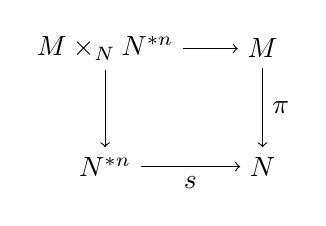
\begin{tikzpicture}[x=20mm,y=15mm]
		\node (a) at (0,0) {$M \times_{\mathbb{N}} \mathbb{N}^{*n}$};
		\node (b) at (1,0) {$M$};
		\node (c) at (0,-1) {$\mathbb{N}^{*n}$};
		\node (d) at (1,-1) {$\mathbb{N}$};
			\draw [->] (a) to node [above] {$$} (b);
			\draw [->] (b) to node [right] {$\pi$} (d);
			\draw [->] (a) to node [left] {$$} (c);
			\draw [->] (c) to node [below] {$s$} (d);
    \end{tikzpicture}
\end{center}
is also a free monoid, where the map $s:\mathbb{N}^{* n} \to \mathbb{N}$ sends every generator to 1.

QQQ Need to make sure we are using the correct notation: the operad, the monad, the monoid, etc
\begin{cor}\label{freemor} 
Let $(M, \pi)$ be as in \cref{Gfree}, and $\mathcal{G}$ a generating set of indivisible elements. Then the monoid $M \times_{\mathbb{N}} \mathbb{N}^{*n}$ is free on
\[
\sum_{k= 0}^{\infty} n^k |\mathcal{G}_k|
\]
generators, where $\mathcal{G}_k \subset \mathcal{G}$ consists of all generators $g \in \mathcal{G}$ such that $\pi(g) =k$.

We can now use these results to express the monoid $\mathrm{Mor}(\ELn)$ using generators for the action operad $\ML$.

\begin{prop} \label{freemor} Let $\mathcal{G}$ be a set that freely generates the action operad $\ML$ under tensor product, and for each $m \in \mathbb{N}$ define $\mathcal{G}_m := \mathcal{G} \, \cap \,  \Lambda(m)$, the subset of $\mathcal{G}$ containing all elements of length $m$. Then the monoid $\mathrm{Mor}(\ELn)$ is 
\[ \ML \times_{\mathbb{N}} \mathbb{N}^{\ast n} \quad = \quad \mathbb{N}^{\ast ( \, |\mathcal{G}_0| + n|\mathcal{G}_1| + n^2 |\mathcal{G}_2| + ... \, )} \]
\end{prop}
%Assume that an action operad $\ML$ is free as a monoid under tensor product on the set $\mathcal{G}$, and define $\mathcal{G}_k := \mathcal{G} \, \cap \,  \Lambda(k)$. Then the monoid of morphisms of the free $\ML$-monoidal category on $n$ generators, $ (\ML, \otimes) \times_{\mathbb{N}} \mathbb{N}^{\ast n}$, is free on 
%\[
%\sum_{k= 0}^{\infty} n^k |\mathcal{G}_k|
%\]
%generators.
%
%Let $\mathcal{G}$ be a set that freely generates the action operad $G$ under tensor product, and for each $m \in \mathbb{N}$ define $\mathcal{G}_m := \mathcal{G} \, \cap \,  G(m)$, the subset of $\mathcal{G}$ containing all elements of length $m$. Then the monoid $\mathrm{Mor}(\ELn)$ is 
%\[ G \times_{\mathbb{N}} \mathbb{N}^{\ast n} \quad = \quad \mathbb{N}^{\ast ( \, |\mathcal{G}_0| + n|\mathcal{G}_1| + n^2 |\mathcal{G}_2| + ... \, )} \]
\end{cor}
\begin{proof}
Let $(g, w)$ be an arbitrary element of $\ML \times_{\mathbb{N}} \mathbb{N}^{\ast n}$. The monoid $\ML$ is free of the generators $\mathcal{G}$, and $\mathbb{N}^{\ast n}$ is free on $\{z_1, ..., z_n\}$, so we can find unique expansions of $g$ and $w$ as tensor products
Let $(m, w)$ be an arbitrary element of $M \times_{\mathbb{N}} \mathbb{N}^{\ast n}$. The monoid $M$ is free of the generators $\mathcal{G}$, and $\mathbb{N}^{\ast n}$ is free on $\{z_1, ..., z_n\}$, so we can find unique expansions of $g$ and $w$ as products
\[ \begin{array}{rclcrcl}
			g & = & g_1 \otimes ... \otimes g_k, & \quad & g_1, ..., g_k & \in & \mathcal{G} \\
			w & = & x_1 \otimes ... \otimes x_m, & \quad & x_1, ..., x_m & \in & \{z_1, ..., z_n\}
			g & = & g_1 g_2 \cdots g_k, & \quad & g_1, ..., g_k & \in & \mathcal{G} \\
			w & = & x_1 x_2 \cdots x_m, & \quad & x_1, ..., x_m & \in & \{z_1, ..., z_n\}
		\end{array}
\]
But each of the generators $z_1, ..., z_n$ has length 1, so the index $m$ here is really just the length $|w|$, which by the definition of $\ML \times_{\mathbb{N}} \mathbb{N}^{\ast n}$ is also the length $|g| = |g_1| + ... + |g_k|$. Therefore we may write
Each of the generators $z_1, ..., z_n$ maps to 1 via $s$, so $\pi(g)$ is just the length $|w|$. Since $\pi$ is a homomorphism, we also have $\pi(g) = \pi(g_1) + ... + \pi(g_k)$. Write $\pi(\leq i)$ for the sum $\pi(g_1) + \cdots + \pi(g_i)$. We then have the equalities
\[ \begin{array}{rll}
			(g, w) & = & (g_1 \otimes ... \otimes g_k, x_1 \otimes ... \otimes x_{|w|}) \\
			& = & (g_1, x_1 \otimes ... \otimes x_{|g_1|}) \otimes (g_2, x_{|g_1|+1} \otimes ... \otimes x_{|g_1|+|g_2|}) \otimes ... \\
			& & \otimes (g_k, x_{|g_1| + ... + |g_{k-1}|+1} \otimes ... \otimes x_{|g_1| + ... + |g_k|})
			(g, w) & = & ( g_1 g_2 \cdots g_k, x_1 x_2 \cdots x_{|w|}) \\
			& = & (g_1, x_1 \cdots x_{\pi(g_1)}) \cdot (g_2, x_{\pi(\leq 1)+1} \cdots x_{\pi(\leq 2)}) \cdot  (g_k, x_{\pi(\leq k-1)+1}\cdots x_{\pi(\leq k)}).
		\end{array}
\]
<<<<<<< Updated upstream
That is, every element in $\ML \times_{\mathbb{N}} \mathbb{N}^{\ast n}$ may be expressed as a product of elements from the subset $\mathcal{G} \times_{\mathbb{N}} \mathbb{N}^{\ast n}$. Furthermore, the freeness of $\ML$ and $\mathbb{N}^{\ast n}$ make sure that this expansion is unique, since
\[ \begin{array}{rl}
			& (g_1, x_1 \otimes ... x_{|g_1|}) \otimes ... \otimes (g_k, x_{|g_1| + ... + |g_{k-1}|+1} \otimes ... \otimes x_{|g_1| + ... + |g_k|}) \\
@ -1660,21 +1762,44 @@ which is just the $m$-fold free product of $\mathbb{N}$ with itself, where $m$ i
			|\mathcal{G} \times_{\mathbb{N}} \mathbb{N}^{\ast n}| & = & |\mathcal{G}_0| \cdot |\{ z_1, ..., z_n \}^0|  \, + \, |\mathcal{G}_1| \cdot |\{ z_1, ..., z_n \}^1| \, + \, |\mathcal{G}_2| \cdot |\{ z_1, ..., z_n \}^2| \, + \, ... \\
			& = & |\mathcal{G}_0| + n|\mathcal{G}_1| + n^2 |\mathcal{G}_2| + ... 
		\end{array}	
=======
This shows that every element in $M \times_{\mathbb{N}} \mathbb{N}^{\ast n}$ may be expressed as a product of elements from the subset $\mathcal{G} \times_{\mathbb{N}} \mathbb{N}^{\ast n}$. Furthermore, the freeness of $M$ and $\mathbb{N}^{\ast n}$ make sure that this expansion is unique, so $M \times_{\mathbb{N}} \mathbb{N}^{\ast n}$ is free on
\[
\mathcal{G} \times_{\mathbb{N}} \mathbb{N}^{\ast n} = \coprod_{k \geq 1} \mathcal{G}_k \times \{z_1, \ldots, z_n \}^k.
>>>>>>> Stashed changes
\]
\end{proof}

This makes the group completion and abelianization we want to do trivial. 
%since
%\[ \begin{array}{rl}
%			& (g_1, x_1 \otimes ... x_{|g_1|}) \otimes ... \otimes (g_k, x_{|g_1| + ... + |g_{k-1}|+1} \otimes ... \otimes x_{|g_1| + ... + |g_k|}) \\
%			= & (g'_1, x'_1 \otimes ... \otimes x'_{|g'_1|}) \otimes ... \otimes (g'_{k'}, x'_{|g'_1| + ... + |g'_{k'-1}|+1} \otimes ... \otimes x'_{|g'_1| + ... + |g'_{k'}|})
%		\end{array}
%\]
%\[ \begin{array}{rcclcccl}
%			\implies \quad \quad & g_1 \otimes ... \otimes g_k & = & g'_1 \otimes ... \otimes g'_{k'}, & \quad \quad & x_1 \otimes ... \otimes x_{m} & = & x'_1 \otimes ... \otimes x'_{m'} \\
%			& & & & & & & \\
%			\implies \quad \quad & g_i \, = \, g'_i, & & 1 \le i \le k = k', & \quad \quad & x_j \, = \, x'_j, & & 1 \le j \le m = m' 
%		\end{array}
%\]
%Thus $G \times_{\mathbb{N}} \mathbb{N}^{\ast n}$ is the free monoid on the set 
%\[ \mathcal{G} \times_{\mathbb{N}} \mathbb{N}^{\ast n} \quad = \quad \mathcal{G}_0 \times \{ z_1, ..., z_n \}^0  \, \cup \, \mathcal{G}_1 \times \{ z_1, ..., z_n \}^1 \, \cup \, \mathcal{G}_2 \times \{ z_1, ..., z_n \}^2 \, \cup \, ...\]
%which is just the $m$-fold free product of $\mathbb{N}$ with itself, where $m$ is the number of generators,
%\[ \begin{array}{rll}
%			|\mathcal{G} \times_{\mathbb{N}} \mathbb{N}^{\ast n}| & = & |\mathcal{G}_0| \cdot |\{ z_1, ..., z_n \}^0|  \, + \, |\mathcal{G}_1| \cdot |\{ z_1, ..., z_n \}^1| \, + \, |\mathcal{G}_2| \cdot |\{ z_1, ..., z_n \}^2| \, + \, ... \\
%			& = & |\mathcal{G}_0| + n|\mathcal{G}_1| + n^2 |\mathcal{G}_2| + ... 
%		\end{array}	
%\]
\end{proof}

\begin{cor} \label{freemorgpab} If $\mathcal{G}$ is a set that freely generates $\ML$ under tensor product, and $\mathcal{G}_m := \mathcal{G} \, \cap \,  \Lambda(m)$, then the abelian group $\mathrm{Mor}(\ELn)^{\mathrm{gp}, \mathrm{ab}}$ is 
\[ (\ML \times_{\mathbb{N}} \mathbb{N}^{\ast n})^{\mathrm{gp}, \mathrm{ab}} \quad = \quad \mathbb{Z}^{|\mathcal{G}_0| + n|\mathcal{G}_1| + n^2 |\mathcal{G}_2| + ...}. \]
\begin{cor}\label{cor:ML_free}
If $\ML$ is an action operad with trivial $\Lambda(0)$, then both $(\ML, \otimes)$ and $\mathrm{Mor}(\ELn) = (\ML, \otimes) \times_{\mathbb{N}} \mathbb{N}^{\ast n}$  are free monoids under tensor product.
\end{cor}
\begin{proof}
The first statement follows from \cref{Gfree} and the proof of \cref{cqr}, and then the second is a consequence of the first and \cref{freemor}.

%Now all that remains is to account for what happens when we collapse the morphisms of $\ELn$ --- that is, evaluate the quotient
%\[ \mathrm{M}(\ELn)^{\mathrm{gp}, \mathrm{ab}} \quad = \quad \bigquotient{\mathbb{Z}^{|\mathcal{G}_0| + n|\mathcal{G}_1| + n^2 |\mathcal{G}_2| + ...}}{\otimes \sim \circ} \]
%Unfortunately, because this will depend on the exact multiplicative structure of the operad groups $G(m)$, there is no way to carry out this computation in general. The best we can say is that as composition in $\mathrm{Mor}(\ELn)$ is partly determined by the group multiplication of the $G(m)$, then in place of $\mathcal{G}$ in the quotient in \cref{freemorgpab} it would suffice to have some collection of elements which generate $G$ when using multiplication as well as tensor product.

If we use a subset $\mathcal{G}' \subseteq \mathcal{G}$ which generates $\ML$ using both the tensor product and group multiplication, then we can reduce the number of generators even further.
\end{proof}

<<<<<<< Updated upstream
\begin{cor} Let $\mathcal{G}$ be a subset of the action operad $\ML$ that freely generates it under tensor product, and let $\mathcal{G'}$ be a subset of $\mathcal{G}$ which generates $\ML$ under a combination of tensor product and group multiplication. Also let $\mathcal{G}_m := \mathcal{G} \, \cap \,  G(m)$ and $\mathcal{G}'_m := \mathcal{G}' \, \cap \,  G(m)$. Then

\[ \bigquotient{\mathbb{Z}^{|\mathcal{G}_0| + n|\mathcal{G}_1| + n^2 |\mathcal{G}_2| + ...}}{\otimes \sim \circ} \quad \quad \cong \quad \quad \bigquotient{\mathbb{Z}^{|\mathcal{G}'_0| + n|\mathcal{G}'_1| + n^2 |\mathcal{G}'_2| + ...}}{\otimes \sim \circ} \]
@ -1698,15 +1823,253 @@ Therefore any generator $(g, w) \in \mathcal{G} \times_{\mathbb{N}} \mathbb{N}^{

%Beyond this, the value of this quotient will have to be found separately for each individual action operad. 

=======
\cref{cor:ML_free} makes the group completion and abelianization we want to compute trivial. 

\section{A full description of \texorpdfstring{$L_n$}{L_n}}
\begin{cor} \label{freemorgpab} If $\mathcal{G}$ is a set that freely generates $(\ML, \otimes)$ under tensor product, and $\mathcal{G}_k := \mathcal{G} \, \cap \,  \Lambda(k)$, then the abelian group $\mathrm{Mor}(\ELn)^{\mathrm{gp}, \mathrm{ab}}$ is 
\[ (G \times_{\mathbb{N}} \mathbb{N}^{\ast n})^{\mathrm{gp}, \mathrm{ab}} \quad = \quad \mathbb{Z}^{|\mathcal{G}_0| + n|\mathcal{G}_1| + n^2 |\mathcal{G}_2| + ...} \]
\end{cor}

QQQ start here. Is the rest of this section necessary/useful?

Now all that remains is to account for what happens when we collapse the morphisms of $\ELn$ --- that is, evaluate the quotient
\[ \mathrm{M}(\ELn)^{\mathrm{gp}, \mathrm{ab}} \quad = \quad \bigquotient{\mathbb{Z}^{|\mathcal{G}_0| + n|\mathcal{G}_1| + n^2 |\mathcal{G}_2| + ...}}{\otimes \sim \circ} \]
Unfortunately, because this will depend on the exact multiplicative structure of the operad groups $G(m)$, there is no way to carry out this computation in general. The best we can say is that as composition in $\mathrm{Mor}(\ELn)$ is partly determined by the group multiplication of the $G(m)$, then in place of $\mathcal{G}$ in the quotient in \cref{freemorgpab} it would suffice to have some collection of elements which generate $G$ when using multiplication as well as tensor product.

\begin{lem} Let $\mathcal{G}$ be a subset of the action operad $G$ that freely generates it under tensor product, and let $\mathcal{G'}$ be a subset of $\mathcal{G}$ which generates $G$ under a combination of tensor product and group multiplication. Also let $\mathcal{G}_m := \mathcal{G} \, \cap \,  G(m)$ and $\mathcal{G}'_m := \mathcal{G}' \, \cap \,  G(m)$. Then

\[ \bigquotient{\mathbb{Z}^{|\mathcal{G}_0| + n|\mathcal{G}_1| + n^2 |\mathcal{G}_2| + ...}}{\otimes \sim \circ} \quad \quad = \quad \quad \bigquotient{\mathbb{Z}^{|\mathcal{G}'_0| + n|\mathcal{G}'_1| + n^2 |\mathcal{G}'_2| + ...}}{\otimes \sim \circ} \]
\end{lem}
\begin{proof} 
Compostion in $\mathrm{Mor}(\ELn)$ is given by
\[ \alpha(g'; \mathrm{id}_{x_{\pi(g^{-1})(1)}}, ..., \mathrm{id}_{x_{\pi(g^{-1})(m)}}) \, \circ \, \alpha(g; \mathrm{id}_{x_1}, ..., \mathrm{id}_{x_m}) \quad = \quad \alpha(g'g; \mathrm{id}_{x_1}, ..., \mathrm{id}_{x_m})\]
which in $G \times_{\mathbb{N}} \mathbb{N}^{\ast n}$ terms is
\[ \big( \, g', \pi(g^{-1})(w) \, \big) \, \circ \, (g, w) \quad = \quad (g'g, w) \]
Thus any element $(g, w)$ of $\mathcal{G} \times_{\mathbb{N}} \mathbb{N}^{\ast n}$ can be expressed in terms of elements of $\mathcal{G}' \times_{\mathbb{N}} \mathbb{N}^{\ast n}$ by way of tensor product and compostion. All we need to do is find and expansion for $g$ using $\mathcal{G}'$, and then pull all of the multiplication and tensors outside of the brackets via the equation above and those we employed back in \cref{freemon}. This means that when we take the quotient by the relation $\otimes \sim \circ$, the equivalence class for $(g, w)$ will be a tensor product of equivalence classes of elements from $\mathcal{G}' \times_{\mathbb{N}} \mathbb{N}^{\ast n}$. In other words, every generator of $\mathbb{Z}^{|\mathcal{G}_0| + n|\mathcal{G}_1| + n^2 |\mathcal{G}_2| + ...}/\otimes \sim \circ$ is contained within the subgroup coming from $\mathcal{G}'$, and therefore so is the whole of the group. That is, 
\[ \begin{array}{rcl}
			\bigquotient{\mathbb{Z}^{|\mathcal{G}_0| + n|\mathcal{G}_1| + n^2 |\mathcal{G}_2| + ...}}{\otimes \sim \circ} \quad & = & \quad \bigquotient{\mathbb{Z}^{|\mathcal{G}' \, \cap \, \mathcal{G}_0| + n|\mathcal{G}' \, \cap \, \mathcal{G}_1| + n^2 |\mathcal{G}' \, \cap \, \mathcal{G}_2| + ...}}{\otimes \sim \circ} \\
			& = & \quad \bigquotient{\mathbb{Z}^{|\mathcal{G}'_0| + n|\mathcal{G}'_1| + n^2 |\mathcal{G}'_2| + ...}}{\otimes \sim \circ}
		\end{array}
\]
\end{proof}

Beyond this, the value of this quotient will have to be found separately for each individual action operad. 

\section{The operad action on \texorpdfstring{$L_n$}{L_n}}

We have determined the monoid of objects of $L_n$ in QQQ, and the abelian group of automorphisms of the unit $L_n(I,I)$ combining QQQ, all that remains is to explicitly construct $L_n$ as a $\ML$-monoidal category. Thus we turn to equipping the underlying groupoid we have constructed with an $E\Lambda$-action. For this, we will exploit the required surjectivity of the $\ML$-monoidal functor $\ELnn \to L_n$ from  \cref{qsurj} and express the operad action on $L_n$ in terms of the operad action on $\ELnn$.

Recall that $\zz^{*n}$ (on generators $g_1, \ldots, g_n$) is a quotient of the free monoid $\nn^{*2n}$ (on generators $m_1, \ldots, m_{2n}$) by the relation setting $m_i m_{n+i} = 1 = m_{n+i} m_i$; then $g_i$ is the image of $m_i$, and $g_i^{-1}$ is the image of $m_{n+i}$. If we write $q$ for the quotient homomorphism $\nn^{*2n} \to \zz^{*n}$, then $q$ has a canonical section $s$ (which is just a function, and not a monoid homomorphism) described as follows. Every element of $\zz^{*n}$ can be written uniquely in normal form as a word $w = w_1 w_2 \cdots w_k$ of minimal length, where each $w_j \in \{g_1^{\pm 1}, \ldots, g_m^{\pm 1}\}$. Then define $s(w) = s(w_1) \cdot s(w_2) \cdots s(w_k)$ by
\[
s(w_j) = \left\{
\begin{array}{rcl}
m_i & \textrm{if} & w_j = g_i, \\
m_{n+i} & \textrm{if} & w_j = g_i^{-1}.
\end{array} \right.
\]

\begin{prop}\label{crossact}
Let $\ML$ be a crossed action operad, $m \in \nn$, $g \in \Lambda(m)$, and $x_1, \ldots, x_m \in \mathrm{Ob}(L_n) $. Then the morphism 
\[
g^{\otimes}: x_1 \otimes \cdots x_m \to x_{\pi(g^{-1})(1)} \otimes \cdots \otimes x_{\pi(g^{-1})(m)}
\]
in $L_n$ is given by 
\[
\Psi \Big( g^{\otimes}: s(x_1) \otimes \cdots s(x_m) \to s(x_{\pi(g^{-1})(1)}) \otimes \cdots \otimes s(x_{\pi(g^{-1})(m)}) \Big)
\]
where $\Psi: \mathrm{Mor}(\ELnn) \to L_n(I,I)$ is composite
\[
\mathrm{Mor}(\ELnn) \to \mathrm{M}(\ELnn)^{\mathrm{gp}, \mathrm{ab}} \to \bigquotient{\mathrm{M}(\ELnn)^{\mathrm{gp}, \mathrm{ab}}}{\Delta} \to L_n(I,I)
\] 
of the homomorphisms from QQQ ref, ref, and ref.
\end{prop}
\begin{proof}

The source and target of $g^{\otimes}$ are $x_1 \otimes ... \otimes x_m$ and $x_{\pi(g^{-1})(1)} \otimes ... \otimes x_{\pi(g^{-1})(m)}$ by definition, so to see this morphism as an element of the monoid
\[ \mathrm{Mor}(L_n) \quad \cong \quad (s \times t)(L_n) \times L_n(I,I) \]
we only need to compute its projection onto $L_n(I,I)$. By \cref{qsurj}, $q: \ELnn \to L_n$ is a surjective map of $E\Lambda$-algebras, so 
\[
q\Big( g^{\otimes}_{\ELnn}:s(x_1) \otimes \cdots s(x_m) \to s(x_{\pi(g^{-1})(1)}) \otimes \cdots \otimes s(x_{\pi(g^{-1})(m)}) \Big) = g^{\otimes}_{L_n}.
\]
If we write $p_I:  \mathrm{Mor}(L_{n}) \to L_{n}(I,I)$ for the projection onto the automorphisms of the unit, we will therefore have
$p_I q (g^{\otimes}_{\ELnn}) = p_I(g^{\otimes}_{L_n})$.

Next consider the diagram
\[ \begin{tikzcd}
\mathrm{Mor}(\ELnn) \ar[rr, "\mathrm{Mor}(q)"] \ar[dd] & & \mathrm{Mor}(L_n) \ar[d, "\mathrm{ab}"] \ar[rr, "p_I"] & &  L\mathbb{G}_{n}(I,I) \ar[d, "\cong"] \\
& & \mathrm{Mor}(L_n)^{\mathrm{ab}} \ar[d] \ar[rr] & & \bigquotient{\mathrm{Mor}{L_{n})^{\mathrm{ab}}}}{(s \times t)(L_n)^{\mathrm{ab}}} \ar[d, "\cong"] \\
\mathrm{M}(\ELnn)^{\mathrm{gp},\mathrm{ab}} \ar[rr, swap, "\mathrm{M}(q)^{\mathrm{gp},\mathrm{ab}}"] & & \mathrm{M}(L_n)^{\mathrm{gp},\mathrm{ab}} \ar[rr] & & \bigquotient{\mathrm{M}(L_{n})^{\mathrm{gp}, \mathrm{ab}}}{\mathbb{Z}^{{n}\choose{2}}}
\end{tikzcd} \]
where all unlabelled arrows are the appropriate quotient maps. The region on the left commutes by naturality of the units for the group completion and abelianization adjunctions, and the bottom-right square is the third isomorphism theorem for groups in for the form
\[
\bigquotient{\mathrm{Mor}(L\mathbb{G}_{n})^{\mathrm{ab}}}{(s \times t)(L_n)^{\mathrm{ab}}} \cong\frac{ \displaystyle  \left(\mathrm{Mor}(L\mathbb{G}_{n})^{\mathrm{ab}}/\mathrm{Ob}(L\mathbb{G}_{n})^{\mathrm{ab}} \right)}{ \displaystyle \left( (s \times t)(L_n)^{\mathrm{ab}}/\mathrm{Ob}(L\mathbb{G}_{n})^{\mathrm{ab}} \right)} \cong \bigquotient{\mathrm{M}(L\mathbb{G}_{n})^{\mathrm{gp}, \mathrm{ab}}}{\mathbb{Z}^{{n}\choose{2}}}.
\]

%\[ \begin{array}{rllll}
			%\bigquotient{\mathrm{Mor}(L\mathbb{G}_{n})^{\mathrm{ab}}}{(s \times t)(L_n)^{\mathrm{ab}}} & = & \frac{ \displaystyle  \left(\mathrm{Mor}(L\mathbb{G}_{n})^{\mathrm{ab}}/\mathrm{Ob}(L\mathbb{G}_{n})^{\mathrm{ab}} \right)}{ \displaystyle \left( (s \times t)(L_n)^{\mathrm{ab}}/\mathrm{Ob}(L\mathbb{G}_{n})^{\mathrm{ab}} \right)} & = & \bigquotient{\mathrm{M}(L\mathbb{G}_{n})^{\mathrm{gp}, \mathrm{ab}}}{\mathbb{Z}^{{n}\choose{2}}}
		%\end{array}
%\]
As for the square on the top-right, recall the split extension of groups from \cref{splitex}.
\begin{center}
\begin{tikzpicture}[x=15mm,y=25mm]
  \draw[tikzob,mm] %objects
  (0,0) node (a) {L_n(I,I)}
  (2,0) node (b) {\mathrm{Mor}(L_n)}
  (4,0) node (c) {(s \times t)(L_n)};
\path[->,auto,mm] %arrows;  have to use this instead of tikzar, 
                    % for some reason
  (a) edge node {} (b)
  (b) edge[swap] node {s \times t} (c)
  (c) edge[swap, bend right=35] node {i} (b);
\end{tikzpicture}
\end{center}
By the proof of \cref{splitex}, the specific isomorphism we are using is

\[ \begin{array}{rll}
			\morln & \cong & (s \times t)(L_n) \times L_n(I,I) \\
			f & \mapsto & \Big( \, s(f), \, t(f), \, f \otimes i\big( \, s(f), t(f) \, \big)^* \, \Big)
		\end{array}
\]

so $p_I(f) = f \otimes i\big( \, s(f), t(f) \, \big)^*$, which gives the commutativity of the top right square.
Thus all of the regions within the diagram commute, and hence so will the outside. Thus $p_I \circ q$ is equal to the composite along the left, bottom, and then right edges, which by QQQ refs is $\Psi$. 
>>>>>>> Stashed changes


<<<<<<< Updated upstream
We now give our most complete description of the free $\ML$-monoidal category generated by $n$ invertible objects. We know that an arbitrary morphism of $L_n$ can be described using its source, target, and an element of $L_n(I,I)$. We use this knowledge, together with a chosen isomorphism $\mathrm{Mor}(L_n) \cong (s \times t)(L_n) \times L_n(I,I)$, to write down $L_n$ as a $\ML$-monoidal category.

\begin{conv}
Recall that we have fixed an isomorphism $\mathrm{Mor}(L_n) \cong (s \times t)(L_n) \times L_n(I,I)$ as per \cref{morprod}. Further, assume that $\Lambda(0)$ is the trivial group; if not, replace $\Lambda$ with the action operad $\Lambda'$ of \cref{noscalarcross}.
\end{conv}

=======
%%\[ \begin{tikzcd}
%%L_n(I,I) \ar[r, hookrightarrow] & \mathrm{Mor}(L_n) \ar[r, shift left, "s \times t"] & (s \times t)(L_n) \ar[l, shift left, hookrightarrow, "i"]
%%\end{tikzcd} \]
 %But the monoid $\mathrm{Mor}(L_{n})^{\mathrm{ab}}/(s \times t)(L_n)^{\mathrm{ab}}$ is exactly what we get when we quotient out by those representatives, so we see that
%\[ \begin{array}{rll}
			%[\mathrm{ab}(f)] & = &  [\mathrm{ab}(f)] \otimes \Big[ \mathrm{ab}\Big( \, i\big( \, s(f), t(f) \, \big)^* \, \Big) \, \Big] \\
			%& = & \Big[ \, \mathrm{ab}\Big( \, f \otimes i\big( \, s(f), t(f) \, \big)^* \, \Big) \, \Big] \\
			%& = & \mathrm{ab}\big( \, p_I(f) \, \big) \\
			%& = & p_I(f)
		%\end{array}
%\]
%Here we've used that fact that the equivalence class of a unit endomorphism under the quotient map $\mathrm{Mor}(L_n)^{\mathrm{gp},\mathrm{ab}} \to \mathrm{Mor}(L\mathbb{G}_{n})^{\mathrm{ab}}/(s \times t)(L_n)^{\mathrm{ab}} = L_n(I,I)$ is just the same endomorphism again, and also that $L_n(I,I)^{\mathrm{ab}} = L_n(I,I)$. 


\end{proof}

%
%At this stage, there is only one part of this $E\Lambda$-algebra that we have yet to find --- its action, $\alpha_{L_n}$. When our action operad $G$ is $G(1)$-generated, everything is so simple that there is really only one thing the action could be.
%
%\begin{lem} \label{G1act} Let $G$ be a $G(1)$-generated action operad, $g$ an element of $G(m)$ for some $m \in \mathbb{N}$, and $x_1, ..., x_m$ elements of $\mathbb{Z}^{\ast n}$. Then the action of $L_n$ is given by
%\[ \alpha_{L_n}( \, g \, ; \, \mathrm{id}_{x_1}, ..., \mathrm{id}_{x_m} \, ) \quad = \quad \mathrm{id}_{x_1 \otimes ... \otimes x_m} \]
%\end{lem}
%\begin{proof}
%In order for $\alpha_{L_n}$ to be a well-defined $E\Lambda$-action, the map $\alpha_{L_n}(g; \mathrm{id}_{x_1}, ..., \mathrm{id}_{x_m})$ needs to have source $x_1 \otimes ... \otimes x_m$ and target $x_{\pi(g^{-1})(1)} \otimes ... \otimes x_{\pi(g^{-1})(m)}$, where by non-crossedness of $G$ the latter is also $x_1 \otimes ... \otimes x_m$. But we know from \cref{trivendo} that all morphisms in this $L_n$ are identities, and hence we get the result.
%\end{proof}
%For crossed $G$, things are more complicated. What we need to do is employ the trick that was previously mentioned in \cref{actmorLGn}, where we exploit the surjectivity of the algebra map $q: \ELnn \to L_n$. This will allow us to express $\alpha_{L_n}$ in terms of the action $\alpha_{\ELnn}$.

%\begin{prop} \label{crossact_orig} Let $G$ be a crossed action operad, and for some $m \in \mathbb{N}$ choose an element $g \in G(m)$ and morphisms $(x_1, y_1, h_1), ..., (x_m, y_m, h_m)$ in $L_n$. That is, the $(x_i, y_i)$ are pairs of objects from $(s \times t)(L_n)$, and the $h_i$ are morphisms in $L_n(I,I)$. Then the action of $L_n$ is given by
%\[ \begin{array}{c}
			%\alpha_{L_n}\big( \, g \, ; \, (x_1, y_1, h_1), ..., (x_m, y_m, h_m) \, \big) \\
			%= \\
			%\big( \, \, \bigotimes_i x_i, \quad \bigotimes_i y_{\pi(g^{-1})(i)}, \quad \Psi \alpha_{\ELnn}( \, g \, ; \, \mathrm{id}_{q^{-1}(y_1)}, ..., \mathrm{id}_{q^{-1}(y_m)} \, \, ) \, \otimes \, (\bigotimes_i h_i) \, \big) 
		%\end{array}
%\]
%Here $q^{-1}: \mathrm{Ob}(L_n) \to \mathrm{Ob}(\ELnn)$ is the function 
%\[ \begin{array}{rcrcl}
			%q^{-1} & : & \mathbb{Z}^{\ast n} & \to & \mathbb{N}^{\ast 2n} \\
			%& : & z_i & \mapsto & z_i \\
			%& : & z_i^* & \mapsto & z_{n+i} \\
			%& : & w & \mapsto & \bigotimes_{i=1}^{|w|} \, q^{-1}\big( \, d(w, i) \, \big)
		%\end{array}
%\]
%with $\bigotimes_{i=1}^{|w|} d(w, i)$ the decomposition of $w$ given in \cref{decompdef}, and $\Psi: \mathrm{Mor}(\ELnn) \to L_n(I,I)$ is the canonical map associated with the repeated quotient
%\[ \begin{tikzcd}
%\mathrm{Mor}(\ELnn) \ar[r] & \mathrm{M}(\ELnn)^{\mathrm{gp}, \mathrm{ab}} \ar[r] & \bigquotient{\mathrm{M}(\ELnn)^{\mathrm{gp}, \mathrm{ab}}}{\Delta} \ar[d, equals] & \\
%& & \mathrm{M}(L_{n})^{\mathrm{gp}, \mathrm{ab}} \ar[r] & \bigquotient{\mathrm{M}(L_{n})^{\mathrm{gp}, \mathrm{ab}}}{\mathbb{Z}^{{n}\choose{2}}} \ar[d, equals] \\
%& & & L_n(I,I)
%\end{tikzcd} \]
%\end{prop} 
%\begin{proof}
%%Firstly, by the rules governing $E\Lambda$-actions and \cref{tenscomp}, we know that
%%\[ \begin{array}{rl} 
%%			& \alpha_{L_n}\big( \, g \, ; \, (x_1, y_1, h_1), ..., (x_m, y_m, h_m) \, \big) \\
%%			= & \alpha_{L_n}( \, g \, ; \, \mathrm{id}_{y_1}, ..., \mathrm{id}_{y_m} \, ) \circ \big( \, (x_1, y_1, h_1) \otimes ... \otimes (x_m, y_m, h_m) \, \big) \\
%%			= & \alpha_{L_n}( \, g \, ; \, \mathrm{id}_{y_1}, ..., \mathrm{id}_{y_m} \, ) \circ ( \, x_1 \otimes ... \otimes x_m, \, y_1 \otimes ... \otimes y_m, \, h_1 \otimes ... \otimes h_m \, ) \\
%%			= & \alpha_{L_n}( \, g \, ; \, \mathrm{id}_{y_1}, ..., \mathrm{id}_{y_m} \, ) \otimes \mathrm{id}_{y_1 \otimes ... \otimes y_m}^* \otimes ( \, x_1 \otimes ... \otimes x_m, \, y_1 \otimes ... \otimes y_m, \, h_1 \otimes ... \otimes h_m \, ) \\
%%		\end{array}
%%\]
%%Since we already understand tensor products of objects and unit endomorphisms, we now only need to find the action morphisms on identities. Moreover, we know that the source and target of $\alpha_{L_n}(g; \mathrm{id}_{y_1}, ..., \mathrm{id}_{y_m})$ have to be $y_1 \otimes ... \otimes y_m$ and $y_{\pi(g^{-1})(1)} \otimes ... \otimes y_{\pi(g^{-1})(m)}$ respectively, so to see this morphism as an element of the monoid
%%\[ \mathrm{Mor}(L_n) \quad \cong \quad (s \times t)(L_n) \times L_n(I,I) \]
%%all that is left to understand is its projection onto the unit endomorphisms.
%
%%Now, recall that $q: \ELnn \to L_n$ is a surjective map of $E\Lambda$-algebras, so that for any $f_i \in \mathrm{Mor}(L\mathbb{G}_{n})$ there exist $f'_i \in \mathrm{Mor}(\ELnn)$ with $q(f'_i) = f_i$, and hence
%%\[ q\big( \, \alpha_{\ELnn}( \, g \, ; \, f'_1, ..., f'_m \, ) \, \big) \quad = \quad \alpha_{L_n}( \, g \, ; \, f_1, ..., f_m \, ). \]
%%In particular, for the identities $\mathrm{id}_{y_i} \in \mathrm{Mor}(L\mathbb{G}_{n})$ we can choose $\mathrm{id}_{q^{-1}(y_i)} \in \mathrm{Mor}(\ELnn)$, as by design $q(\mathrm{id}_{q^{-1}(y_i)}) = \mathrm{id}_{qq^{-1}(y_i)} = \mathrm{id}_{y_i}$. This means that if we denote by $p_I :  \mathrm{Mor}(L\mathbb{G}_{n}) \to L\mathbb{G}_{n}(I,I)$ the projection onto unit endomorphisms, we will have
%%\[ p_I \big( \, \alpha_{L_n}( \, g \, ; \, \mathrm{id}_{y_1}, ..., \mathrm{id}_{y_m} \, ) \, \big) \quad = \quad  p_I q\big( \, \alpha_{\ELnn}( \, g \, ; \, \mathrm{id}_{q^{-1}(y_1)}, ..., \mathrm{id}_{q^{-1}(y_m)} \, ) \, \big). \]
%
%But $p_I \circ q$ is a map that can be described in a different way. Consider the commutative diagram
%\[ \begin{tikzcd}
%\mathrm{Mor}(\ELnn) \ar[rr, "q"] \ar[dd] & & \mathrm{Mor}(L_n) \ar[d, "\mathrm{ab}"] \ar[rr, "p_I"] & &  L\mathbb{G}_{n}(I,I) \ar[d, equals] \\
%& & \mathrm{Mor}(L_n)^{\mathrm{ab}} \ar[d] \ar[rr] & & \bigquotient{\mathrm{Mor}(L\mathbb{G}_{n})^{\mathrm{ab}}}{(s \times t)(L_n)^{\mathrm{ab}}} \ar[d, equals] \\
%\mathrm{M}(\ELnn)^{\mathrm{gp},\mathrm{ab}} \ar[rr, "\mathrm{M}(q)^{\mathrm{gp},\mathrm{ab}}"] & & \mathrm{M}(L_n)^{\mathrm{gp},\mathrm{ab}} \ar[rr] & & \bigquotient{\mathrm{M}(L\mathbb{G}_{n})^{\mathrm{gp}, \mathrm{ab}}}{\mathbb{Z}^{{n}\choose{2}}}
%\end{tikzcd} \]
%where all unlabelled arrows are the appropriate quotient maps. The region on the left commutes by naturality of the adjoint functor $\mathrm{M}(\, \_ \,)^{\mathrm{gp},\mathrm{ab}}$, and the bottom-right square uses the fact that
%\[ \begin{array}{rllll}
			%\bigquotient{\mathrm{Mor}(L\mathbb{G}_{n})^{\mathrm{ab}}}{(s \times t)(L_n)^{\mathrm{ab}}} & = & \frac{ \displaystyle  \left(\mathrm{Mor}(L\mathbb{G}_{n})^{\mathrm{ab}}/\mathrm{Ob}(L\mathbb{G}_{n})^{\mathrm{ab}} \right)}{ \displaystyle \left( (s \times t)(L_n)^{\mathrm{ab}}/\mathrm{Ob}(L\mathbb{G}_{n})^{\mathrm{ab}} \right)} & = & \bigquotient{\mathrm{M}(L\mathbb{G}_{n})^{\mathrm{gp}, \mathrm{ab}}}{\mathbb{Z}^{{n}\choose{2}}}
		%\end{array}
%\]
%As for the square on the top-right, remember that the split extension of groups
%\[ \begin{tikzcd}
%L_n(I,I) \ar[r, hookrightarrow] & \mathrm{Mor}(L_n) \ar[r, shift left, "s \times t"] & (s \times t)(L_n) \ar[l, shift left, hookrightarrow, ""]
%\end{tikzcd} \]
%was the source of our product description of morphisms of $L_n$. Thus by the proof of \cref{splitex}, the specific isomorphism we are using is
%\[ \begin{array}{rll}
			%\mathrm{Mor}(L_n) & \cong & (s \times t)(L_n) \times L_n(I,I) \\
			%f & \mapsto & \Big( \, s(f), \, t(f), \, f \otimes i\big( \, s(f), t(f) \, \big)^* \, \Big)
		%\end{array}
%\]
%and so the projection $p_I$ is given by tensoring a morphism with the inverse of the representative of its source and target under the inclusion $(s \times t)(L_n) \hookrightarrow \mathrm{Mor}(L_n)$. But the monoid $\mathrm{Mor}(L\mathbb{G}_{n})^{\mathrm{ab}}/(s \times t)(L_n)^{\mathrm{ab}}$ is exactly what we get when we quotient out by those representatives, so we see that
%\[ \begin{array}{rll}
			%[\mathrm{ab}(f)] & = &  [\mathrm{ab}(f)] \otimes \Big[ \mathrm{ab}\Big( \, i\big( \, s(f), t(f) \, \big)^* \, \Big) \, \Big] \\
			%& = & \Big[ \, \mathrm{ab}\Big( \, f \otimes i\big( \, s(f), t(f) \, \big)^* \, \Big) \, \Big] \\
			%& = & \mathrm{ab}\big( \, p_I(f) \, \big) \\
			%& = & p_I(f)
		%\end{array}
%\]
%Here we've used that fact that the equivalence class of a unit endomorphism under the quotient map $\mathrm{Mor}(L_n)^{\mathrm{gp},\mathrm{ab}} \to \mathrm{Mor}(L\mathbb{G}_{n})^{\mathrm{ab}}/(s \times t)(L_n)^{\mathrm{ab}} = L_n(I,I)$ is just the same endomorphism again, and also that $L_n(I,I)^{\mathrm{ab}} = L_n(I,I)$. 
%
%Thus all of the regions within the diagram commute, and hence so will the outside. That is, $p_I \circ q$ is equal to the composite along the left and bottom edges, which is $\Psi$. 
%
%%This means that the projection onto $L_n(I,I)$ of our action on identities is
%%\[ \begin{array}{rll}
			%%p_I \big( \, \alpha_{L_n}( \, g \, ; \, \mathrm{id}_{y_1}, ..., \mathrm{id}_{y_m} \, ) \, \big) & = &  p_I q\big( \, \alpha_{\ELnn}( \, g \, ; \, \mathrm{id}_{q^{-1}(y_1)}, ..., \mathrm{id}_{q^{-1}(y_m)} \, ) \, \big) \\
			%%& = & \Psi \big( \, \alpha_{\ELnn}( \, g \, ; \, \mathrm{id}_{q^{-1}(y_1)}, ..., \mathrm{id}_{q^{-1}(y_m)} \, ) \, \big)
		%%\end{array}
%%\]
%%and therefore the action of $L_n$ is given by
%%\[ \begin{array}{c}
			%%\alpha_{L_n}\big( \, g \, ; \, (x_1, y_1, h_1), ..., (x_m, y_m, h_m) \, \big) \\
			%%= \\
			%%\alpha_{L_n}( \, g \, ; \, \mathrm{id}_{y_1}, ..., \mathrm{id}_{y_m} \, ) \circ \, \bigotimes_i (x_i, y_i, h_i) \\
			%%= \\
			%%\big( \, \bigotimes_i y_i, \, \bigotimes_i y_{\pi(g^{-1})(i)}, \, \Psi \alpha_{\ELnn}( \, g \, ; \, \mathrm{id}_{q^{-1}(y_1)}, ..., \mathrm{id}_{q^{-1}(y_m)} \, ) \, \big) \otimes \, \mathrm{id}_{\otimes_i y_i}^* \otimes ( \, \bigotimes_i x_i, \, \bigotimes_i y_i, \, \bigotimes_i h_i \, ) \\
			%%= \\
			%%\big( \, \, \bigotimes_i x_i, \quad \bigotimes_i y_{\pi(g^{-1})(i)}, \quad \Psi \alpha_{\ELnn}( \, g \, ; \, \mathrm{id}_{q^{-1}(y_1)}, ..., \mathrm{id}_{q^{-1}(y_m)} \, \, ) \, \otimes \, (\bigotimes_i h_i) \, \big) 
		%%\end{array}
%%\]
%%as required.
%\end{proof}

\section{A full description of \texorpdfstring{$L_n$}{L_n}}
We now collect together all the results which give a complete and explicit description of $L_n$.

%With this last proposition proven, the results in this thesis now collectively describe how to construct the free $E\Lambda$-algebras on $n$ invertible objects for most values of $G$. However, since this characterization was discovered by us in such a piecemeal fashion, we will now restate everything in one place, for ease of reading. We'll begin with the non-crossed case, or as much of it as we were able to draw a complete conclusion about.

>>>>>>> Stashed changes
%\begin{thm} \label{freeinvalgG1} Let $G$ be a $G(1)$-generated action operad. Then the free $E\Lambda$-algebra on $n$ invertible objects is just the discrete category
%\[ L_n \quad = \quad \mathbb{Z}^{\ast n} \]
%equipped with a tensor product which is the usual monoid multiplication, and an $E\Lambda$-action given by
@ -1717,17 +2080,31 @@ Recall that we have fixed an isomorphism $\mathrm{Mor}(L_n) \cong (s \times t)(L
%\end{proof}
%
%It is a shame that we were not able to find a formulation for uncrossed $L_n$ in full generality. This will have to be the subject of future research.
<<<<<<< Updated upstream
%
%By contrast, in the case of crossed action operads we were able to achieve a complete description. First, using various results from \cref{colimalgebra,morphisms} we showed that the unit endomorphisms of $L_n$ were isomorphic to a certain quotient of abelian groups, which from now on we will refer to as $A(G,n)$. The long process of calculating this group can now be condensed down into a single definition:

We begin by giving a recipe for constructing the group $L_n(I,I)$ from a presentation of the operad $\ML$.

\begin{Defi} \label{AGndef} Let $\ML$ be a crossed action operad. Choose a subset $\mathcal{G}$ that generates $\ML$ under a combination of tensor product and group multiplication, which itself has subsets $\mathcal{G}_m := \mathcal{G} \, \cap \, \Lambda(m)$. Then for each $n \in \mathbb{N}$, we will denote by $A(\ML,n)$ the abelian group obtained from the free abelian group 
=======

%By contrast, in the case of crossed action operads we were able to achieve a complete description. First, using various results from \cref{colimalgebra,morphisms} we showed that the unit endomorphisms of $L_n$ were isomorphic to a certain quotient of abelian groups, which from now on we will refer to as $A(G,n)$. The long process of calculating this group can now be condensed down into a single definition:

We condense all our results QQQ into the following definition.

\begin{Defi} \label{AGndef} Let $\ML$ be a crossed action operad, and $\ML'$ the action operad defined by $\Lambda'(m) := \Lambda(m)/\Lambda(0)$. Choose a subset $\mathcal{G}$ that generates $\Lambda'$ under a combination of tensor product and group multiplication, which itself has subsets $\mathcal{G}_m := \mathcal{G} \, \cap \, \Lambda'(m)$. Then for each $n \in \mathbb{N}$, we will denote by $A(\ML,n)$ the abelian group obtained from the free abelian group 
>>>>>>> Stashed changes
\[ \mathrm{F}( \mathcal{G} \times_{\mathbb{N}} \mathbb{N}^{\ast 2n}) \quad = \quad \mathbb{Z}^{2n|\mathcal{G}_1| + (2n)^2|\mathcal{G}_2| + ...} \]
via the following steps:
via the following steps.
\begin{enumerate}%[leftmargin=*]
<<<<<<< Updated upstream
\item For all $g, g' \in \mathcal{G}_m$ and $w \in \mathbb{N}^{\ast 2n}$ with $|w| = m$, quotient out by the relation 
\[ (g, w) \, \otimes \, \big( \, g', \pi(g^{-1})(w) \, \big) \quad \sim \quad (g \cdot g', w) \]
=======
\item For all $g, g' \in \Lambda(m)$ and $w \in \mathbb{N}^{\ast 2n}$ with $|w| = m$, quotient out by the relation 
\[ (g, w) \, \otimes \, \big( \, g', \pi(g^{-1})(w) \, \big) \quad \sim \quad (g \cdot g', w). \]
>>>>>>> Stashed changes
\item Quotient out by the subgroup $\Delta$, which is generated by the equivalence classes of elements of the form
\[ \begin{array}{c}
				\big( \, \mu( \, g \, ; \, e_{|\tilde{\delta}(x_1)|}, ..., e_{|\tilde{\delta}(x_m)|} \, ), \, \tilde{\delta}( \, x_1 \otimes ... \otimes x_m \, ) \, \big) \\
@ -1738,19 +2115,19 @@ via the following steps:
where $g \in G(m)$, the $x_i$ are generators of $\mathbb{N}^{\ast 4n}$, and for all $1 \le i \le n$,
\[ \begin{array}{rclcrclcrclcrcl}
			\tilde{\delta}(z_i) & = & z_i, & & \tilde{\delta}(z_{2n+i}) & = & z_i \otimes z_{n+i}, & & \tilde{I}(z_i) & = & z_i, & &\tilde{I}(z_{2n+i}) & = & I,\\
			\tilde{\delta}(z_{n+i}) & = & z_{n+i}, &  & \tilde{\delta}(z_{3n+i}) & = & z_{n+i} \otimes z_i & & \tilde{I}(z_{n+i}) & = & z_{n+i}, & & \tilde{I}(z_{3n+i}) & = & I
			\tilde{\delta}(z_{n+i}) & = & z_{n+i}, &  & \tilde{\delta}(z_{3n+i}) & = & z_{n+i} \otimes z_i & & \tilde{I}(z_{n+i}) & = & z_{n+i}, & & \tilde{I}(z_{3n+i}) & = & I.
			 \end{array}
\] 
\item Choose any $\rho(2) \in \pi^{-1}((1 \, 2))$, and then quotient out by the $\mathbb{Z}^{{n}\choose{2}}$ subgroup generated by the equivalence classes of the elements 
\[ \big( \, \rho(2) \, ; \, z_i, z_j \, \big), \quad \quad 1 \le i < j \le n \]
\[ \big( \, \rho(2) \, ; \, z_i, z_j \, \big), \quad \quad 1 \le i < j \le n. \]
\end{enumerate}
Also, we will use $\Psi: G \times_{\mathbb{N}} \mathbb{N}^{\ast 2n} \to A(G,n)$ to represent the corresponding quotient map. 
We write $\Psi: G \times_{\mathbb{N}} \mathbb{N}^{\ast 2n} \to A(G,n)$ to represent the corresponding quotient map. 
\end{Defi}

With this new notation, the main result of this thesis can be stated quite concisely.
With this notation, our main result can be stated concisely.

\begin{thm}\label{freeinvalgc} Let $G$ be a crossed action operad. Then the free $E\Lambda$-algebra on $n$ invertible objects is the category
\[ L_n \quad = \quad \mathbb{Z}^{\ast n} \times_{\mathbb{Z}^n} \mathbb{Z}^{\ast n}  \, \times \, \mathrm{B}A(G,n) \]
\begin{thm}\label{freeinvalgc} Let $\ML$ be a crossed action operad. Then the free $E\Lambda$-algebra on $n$ invertible objects is the category
\[ L_n \quad = \quad \mathbb{Z}^{\ast n} \times_{\mathbb{Z}^n} \mathbb{Z}^{\ast n}  \, \times \, \mathrm{B}A(\ML,n) \]
equipped with a component-wise tensor product,
\[ (x', y' ,h') \otimes (x, y, h) \, = \, ( \, x' \otimes x, \, y' \otimes y, \, h'h \, ) \]
and the $E\Lambda$-action given in \cref{crossact}:
@ -1762,8 +2139,8 @@ and the $E\Lambda$-action given in \cref{crossact}:
\]
\end{thm}
\begin{proof}
The category $\mathbb{Z}^{\ast n} \times_{\mathbb{Z}^n} \mathbb{Z}^{\ast n} \times \mathrm{B}A(G,n)$ is just the one which has objects $\mathbb{Z}^{\ast n} \times_{\mathbb{Z}^n} \mathbb{Z}^{\ast n}$, morphisms $\mathbb{Z}^{\ast n} \times_{\mathbb{Z}^n} \mathbb{Z}^{\ast n} \times A(G,n)$, and composition 
\[ (y, z , h') \circ (x, y, h) \quad = \quad (x, z, h'h) \]
The category $\mathbb{Z}^{\ast n} \times_{\mathbb{Z}^n} \mathbb{Z}^{\ast n} \times \mathrm{B}A(\ML,n)$ is just the one which has objects $\mathbb{Z}^{\ast n} \times_{\mathbb{Z}^n} \mathbb{Z}^{\ast n}$, morphisms $\mathbb{Z}^{\ast n} \times_{\mathbb{Z}^n} \mathbb{Z}^{\ast n} \times A(\ML,n)$, and composition 
\[ (y, z , h') \circ (x, y, h) \quad = \quad (x, z, h'h). \]
We know that these objects and morphisms are correct by \cref{Zobj,Zmor,nchoose2,freemor,noscalarcross}, and those results also tell us that the monoidal structure is as given above. For composition, it follows from \cref{tenscomp} that
\[ \begin{array}{rll} 
			(y, z , h') \circ (x, y, h) & = & (y, z , h') \otimes \mathrm{id}_{y^*} \otimes (x, y, h) \\